%%%%%%%%%%%%%%%%%%%%%%%%%%%%%%%%%%%%%%%%%
% The Legrand Orange Book
% LaTeX Template
% Version 2.4 (26/09/2018)
%
% This template was downloaded from:
% http://www.LaTeXTemplates.com
%
% Original author:
% Mathias Legrand (legrand.mathias@gmail.com) with modifications by:
% Vel (vel@latextemplates.com)
%
% License:
% CC BY-NC-SA 3.0 (http://creativecommons.org/licenses/by-nc-sa/3.0/)
%
% Compiling this template:
% This template uses biber for its bibliography and makeindex for its index.
% When you first open the template, compile it from the command line with the 
% commands below to make sure your LaTeX distribution is configured correctly:
%
% 1) pdflatex main
% 2) makeindex main.idx -s StyleInd.ist
% 3) biber main
% 4) pdflatex main x 2
%
% After this, when you wish to update the bibliography/index use the appropriate
% command above and make sure to compile with pdflatex several times 
% afterwards to propagate your changes to the document.
%
% This template also uses a number of packages which may need to be
% updated to the newest versions for the template to compile. It is strongly
% recommended you update your LaTeX distribution if you have any
% compilation errors.
%
% Important note:
% Chapter heading images should have a 2:1 width:height ratio,
% e.g. 920px width and 460px height.
%
%%%%%%%%%%%%%%%%%%%%%%%%%%%%%%%%%%%%%%%%%

%----------------------------------------------------------------------------------------
%	PACKAGES AND OTHER DOCUMENT CONFIGURATIONS
%----------------------------------------------------------------------------------------

\documentclass[11pt,fleqn]{book} % Default font size and left-justified equations
\newcommand{\ebeam}{\ensuremath{E_{\mathrm{beam}}}\xspace}
  \newcommand{\pt}{\ensuremath{p_{\mathrm{T}}}\xspace}
    \newcommand{\Lint}{\ensuremath{\mathcal{L}_{\mathrm{int}}}\xspace}
   \newcommand{\ttbar}{\ensuremath{t\bar{t}}\xspace}

%%%%%%%%%%%%%%%%%%%%%%%%%%%%%%%%%%%%%%%%%
% The Legrand Orange Book
% Structural Definitions File
% Version 2.1 (26/09/2018)
%
% Original author:
% Mathias Legrand (legrand.mathias@gmail.com) with modifications by:
% Vel (vel@latextemplates.com)
% 
% This file was downloaded from:
% http://www.LaTeXTemplates.com
%
% License:
% CC BY-NC-SA 3.0 (http://creativecommons.org/licenses/by-nc-sa/3.0/)
%
%%%%%%%%%%%%%%%%%%%%%%%%%%%%%%%%%%%%%%%%%

%----------------------------------------------------------------------------------------
%	VARIOUS REQUIRED PACKAGES AND CONFIGURATIONS
%----------------------------------------------------------------------------------------

\usepackage{amsmath, amsfonts} % Math packages

\usepackage{graphicx} % Required for including pictures
\graphicspath{{Pictures/}} % Specifies the directory where pictures are stored

\usepackage{lipsum} % Inserts dummy text
\usepackage{xspace}
\usepackage{tikz} % Required for drawing custom shapes

\usepackage[english]{babel} % English language/hyphenation

\usepackage{enumitem} % Customize lists
\setlist{nolistsep} % Reduce spacing between bullet points and numbered lists

\usepackage{booktabs} % Required for nicer horizontal rules in tables
\usepackage{subfigure}
\usepackage{xcolor} % Required for specifying colors by name
%\definecolor{ocre}{RGB}{243,102,25} % Define the orange color used for highlighting throughout the book
\definecolor{ocre}{RGB}{0,59,72} % Define the orange color used for highlighting throughout the book

\usepackage{atlasunit}

%----------------------------------------------------------------------------------------
%	MARGINS
%----------------------------------------------------------------------------------------

\usepackage{geometry} % Required for adjusting page dimensions and margins

\geometry{
	paper=a4paper, % Paper size, change to letterpaper for US letter size
	top=3cm, % Top margin
	bottom=3cm, % Bottom margin
	left=3cm, % Left margin
	right=3cm, % Right margin
	headheight=14pt, % Header height
	footskip=1.4cm, % Space from the bottom margin to the baseline of the footer
	headsep=10pt, % Space from the top margin to the baseline of the header
	%showframe, % Uncomment to show how the type block is set on the page
}

%----------------------------------------------------------------------------------------
%	FONTS
%----------------------------------------------------------------------------------------

\usepackage{avant} % Use the Avantgarde font for headings
%\usepackage{times} % Use the Times font for headings
\usepackage{mathptmx} % Use the Adobe Times Roman as the default text font together with math symbols from the Sym­bol, Chancery and Com­puter Modern fonts

\usepackage{microtype} % Slightly tweak font spacing for aesthetics
\usepackage[utf8]{inputenc} % Required for including letters with accents
\usepackage[T1]{fontenc} % Use 8-bit encoding that has 256 glyphs

%----------------------------------------------------------------------------------------
%	BIBLIOGRAPHY AND INDEX
%----------------------------------------------------------------------------------------

\usepackage[style=numeric,citestyle=numeric,sorting=nyt,sortcites=true,autopunct=true,babel=hyphen,hyperref=true,abbreviate=false,backref=true,backend=biber]{biblatex}
\addbibresource{main.bib} % BibTeX bibliography file
\defbibheading{bibempty}{}

\usepackage{calc} % For simpler calculation - used for spacing the index letter headings correctly
\usepackage{makeidx} % Required to make an index
\makeindex % Tells LaTeX to create the files required for indexing

%----------------------------------------------------------------------------------------
%	MAIN TABLE OF CONTENTS
%----------------------------------------------------------------------------------------

\usepackage{titletoc} % Required for manipulating the table of contents

\contentsmargin{0cm} % Removes the default margin

% Part text styling (this is mostly taken care of in the PART HEADINGS section of this file)
\titlecontents{part}
	[0cm] % Left indentation
	{\addvspace{20pt}\bfseries} % Spacing and font options for parts
	{}
	{}
	{}

% Chapter text styling
\titlecontents{chapter}
	[1.25cm] % Left indentation
	{\addvspace{12pt}\large\sffamily\bfseries} % Spacing and font options for chapters
	{\color{ocre!60}\contentslabel[\Large\thecontentslabel]{1.25cm}\color{ocre}} % Formatting of numbered sections of this type
	{\color{ocre}} % Formatting of numberless sections of this type
	{\color{ocre!60}\normalsize\;\titlerule*[.5pc]{.}\;\thecontentspage} % Formatting of the filler to the right of the heading and the page number

% Section text styling
\titlecontents{section}
	[1.25cm] % Left indentation
	{\addvspace{3pt}\sffamily\bfseries} % Spacing and font options for sections
	{\contentslabel[\thecontentslabel]{1.25cm}} % Formatting of numbered sections of this type
	{} % Formatting of numberless sections of this type
	{\hfill\color{black}\thecontentspage} % Formatting of the filler to the right of the heading and the page number

% Subsection text styling
\titlecontents{subsection}
	[1.25cm] % Left indentation
	{\addvspace{1pt}\sffamily\small} % Spacing and font options for subsections
	{\contentslabel[\thecontentslabel]{1.25cm}} % Formatting of numbered sections of this type
	{} % Formatting of numberless sections of this type
	{\ \titlerule*[.5pc]{.}\;\thecontentspage} % Formatting of the filler to the right of the heading and the page number

% Figure text styling
\titlecontents{figure}
	[1.25cm] % Left indentation
	{\addvspace{1pt}\sffamily\small} % Spacing and font options for figures
	{\thecontentslabel\hspace*{1em}} % Formatting of numbered sections of this type
	{} % Formatting of numberless sections of this type
	{\ \titlerule*[.5pc]{.}\;\thecontentspage} % Formatting of the filler to the right of the heading and the page number

% Table text styling
\titlecontents{table}
	[1.25cm] % Left indentation
	{\addvspace{1pt}\sffamily\small} % Spacing and font options for tables
	{\thecontentslabel\hspace*{1em}} % Formatting of numbered sections of this type
	{} % Formatting of numberless sections of this type
	{\ \titlerule*[.5pc]{.}\;\thecontentspage} % Formatting of the filler to the right of the heading and the page number

%----------------------------------------------------------------------------------------
%	MINI TABLE OF CONTENTS IN PART HEADS
%----------------------------------------------------------------------------------------

% Chapter text styling
\titlecontents{lchapter}
	[0em] % Left indentation
	{\addvspace{15pt}\large\sffamily\bfseries} % Spacing and font options for chapters
	{\color{ocre}\contentslabel[\Large\thecontentslabel]{1.25cm}\color{ocre}} % Chapter number
	{}  
	{\color{ocre}\normalsize\sffamily\bfseries\;\titlerule*[.5pc]{.}\;\thecontentspage} % Page number

% Section text styling
\titlecontents{lsection}
	[0em] % Left indentation
	{\sffamily\small} % Spacing and font options for sections
	{\contentslabel[\thecontentslabel]{1.25cm}} % Section number
	{}
	{}

% Subsection text styling (note these aren't shown by default, display them by searchings this file for tocdepth and reading the commented text)
\titlecontents{lsubsection}
	[.5em] % Left indentation
	{\sffamily\footnotesize} % Spacing and font options for subsections
	{\contentslabel[\thecontentslabel]{1.25cm}}
	{}
	{}

%----------------------------------------------------------------------------------------
%	HEADERS AND FOOTERS
%----------------------------------------------------------------------------------------

\usepackage{fancyhdr} % Required for header and footer configuration

\pagestyle{fancy} % Enable the custom headers and footers

\renewcommand{\chaptermark}[1]{\markboth{\sffamily\normalsize\bfseries\chaptername\ \thechapter.\ #1}{}} % Styling for the current chapter in the header
\renewcommand{\sectionmark}[1]{\markright{\sffamily\normalsize\thesection\hspace{5pt}#1}{}} % Styling for the current section in the header

\fancyhf{} % Clear default headers and footers
\fancyhead[LE,RO]{\sffamily\normalsize\thepage} % Styling for the page number in the header
\fancyhead[LO]{\rightmark} % Print the nearest section name on the left side of odd pages
\fancyhead[RE]{\leftmark} % Print the current chapter name on the right side of even pages
%\fancyfoot[C]{\thepage} % Uncomment to include a footer

\renewcommand{\headrulewidth}{0.5pt} % Thickness of the rule under the header

\fancypagestyle{plain}{% Style for when a plain pagestyle is specified
	\fancyhead{}\renewcommand{\headrulewidth}{0pt}%
}

% Removes the header from odd empty pages at the end of chapters
\makeatletter
\renewcommand{\cleardoublepage}{
\clearpage\ifodd\c@page\else
\hbox{}
\vspace*{\fill}
\thispagestyle{empty}
\newpage
\fi}

%----------------------------------------------------------------------------------------
%	THEOREM STYLES
%----------------------------------------------------------------------------------------

\usepackage{amsmath,amsfonts,amssymb,amsthm} % For math equations, theorems, symbols, etc

\newcommand{\intoo}[2]{\mathopen{]}#1\,;#2\mathclose{[}}
\newcommand{\ud}{\mathop{\mathrm{{}d}}\mathopen{}}
\newcommand{\intff}[2]{\mathopen{[}#1\,;#2\mathclose{]}}
\renewcommand{\qedsymbol}{$\blacksquare$}
\newtheorem{notation}{Notation}[chapter]

% Boxed/framed environments
\newtheoremstyle{ocrenumbox}% Theorem style name
{0pt}% Space above
{0pt}% Space below
{\normalfont}% Body font
{}% Indent amount
{\small\bf\sffamily\color{ocre}}% Theorem head font
{\;}% Punctuation after theorem head
{0.25em}% Space after theorem head
{\small\sffamily\color{ocre}\thmname{#1}\nobreakspace\thmnumber{\@ifnotempty{#1}{}\@upn{#2}}% Theorem text (e.g. Theorem 2.1)
\thmnote{\nobreakspace\the\thm@notefont\sffamily\bfseries\color{black}---\nobreakspace#3.}} % Optional theorem note

\newtheoremstyle{blacknumex}% Theorem style name
{5pt}% Space above
{5pt}% Space below
{\normalfont}% Body font
{} % Indent amount
{\small\bf\sffamily}% Theorem head font
{\;}% Punctuation after theorem head
{0.25em}% Space after theorem head
{\small\sffamily{\tiny\ensuremath{\blacksquare}}\nobreakspace\thmname{#1}\nobreakspace\thmnumber{\@ifnotempty{#1}{}\@upn{#2}}% Theorem text (e.g. Theorem 2.1)
\thmnote{\nobreakspace\the\thm@notefont\sffamily\bfseries---\nobreakspace#3.}}% Optional theorem note

\newtheoremstyle{blacknumbox} % Theorem style name
{0pt}% Space above
{0pt}% Space below
{\normalfont}% Body font
{}% Indent amount
{\small\bf\sffamily}% Theorem head font
{\;}% Punctuation after theorem head
{0.25em}% Space after theorem head
{\small\sffamily\thmname{#1}\nobreakspace\thmnumber{\@ifnotempty{#1}{}\@upn{#2}}% Theorem text (e.g. Theorem 2.1)
\thmnote{\nobreakspace\the\thm@notefont\sffamily\bfseries---\nobreakspace#3.}}% Optional theorem note

% Non-boxed/non-framed environments
\newtheoremstyle{ocrenum}% Theorem style name
{5pt}% Space above
{5pt}% Space below
{\normalfont}% Body font
{}% Indent amount
{\small\bf\sffamily\color{ocre}}% Theorem head font
{\;}% Punctuation after theorem head
{0.25em}% Space after theorem head
{\small\sffamily\color{ocre}\thmname{#1}\nobreakspace\thmnumber{\@ifnotempty{#1}{}\@upn{#2}}% Theorem text (e.g. Theorem 2.1)
\thmnote{\nobreakspace\the\thm@notefont\sffamily\bfseries\color{black}---\nobreakspace#3.}} % Optional theorem note
\makeatother

% Defines the theorem text style for each type of theorem to one of the three styles above
\newcounter{dummy} 
\numberwithin{dummy}{section}
\theoremstyle{ocrenumbox}
\newtheorem{theoremeT}[dummy]{Theorem}
\newtheorem{problem}{Problem}[chapter]
\newtheorem{exerciseT}{Exercise}[chapter]
\theoremstyle{blacknumex}
\newtheorem{exampleT}{Example}[chapter]
\theoremstyle{blacknumbox}
\newtheorem{vocabulary}{Vocabulary}[chapter]
\newtheorem{definitionT}{Definition}[section]
\newtheorem{corollaryT}[dummy]{Corollary}
\theoremstyle{ocrenum}
\newtheorem{proposition}[dummy]{Proposition}

%----------------------------------------------------------------------------------------
%	DEFINITION OF COLORED BOXES
%----------------------------------------------------------------------------------------

\RequirePackage[framemethod=default]{mdframed} % Required for creating the theorem, definition, exercise and corollary boxes

% Theorem box
\newmdenv[skipabove=7pt,
skipbelow=7pt,
backgroundcolor=black!5,
linecolor=ocre,
innerleftmargin=5pt,
innerrightmargin=5pt,
innertopmargin=5pt,
leftmargin=0cm,
rightmargin=0cm,
innerbottommargin=5pt]{tBox}

% Exercise box	  
\newmdenv[skipabove=7pt,
skipbelow=7pt,
rightline=false,
leftline=true,
topline=false,
bottomline=false,
backgroundcolor=ocre!10,
linecolor=ocre,
innerleftmargin=5pt,
innerrightmargin=5pt,
innertopmargin=5pt,
innerbottommargin=5pt,
leftmargin=0cm,
rightmargin=0cm,
linewidth=4pt]{eBox}	

% Definition box
\newmdenv[skipabove=7pt,
skipbelow=7pt,
rightline=false,
leftline=true,
topline=false,
bottomline=false,
linecolor=ocre,
innerleftmargin=5pt,
innerrightmargin=5pt,
innertopmargin=0pt,
leftmargin=0cm,
rightmargin=0cm,
linewidth=4pt,
innerbottommargin=0pt]{dBox}	

% Corollary box
\newmdenv[skipabove=7pt,
skipbelow=7pt,
rightline=false,
leftline=true,
topline=false,
bottomline=false,
linecolor=gray,
backgroundcolor=black!5,
innerleftmargin=5pt,
innerrightmargin=5pt,
innertopmargin=5pt,
leftmargin=0cm,
rightmargin=0cm,
linewidth=4pt,
innerbottommargin=5pt]{cBox}

% Creates an environment for each type of theorem and assigns it a theorem text style from the "Theorem Styles" section above and a colored box from above
\newenvironment{theorem}{\begin{tBox}\begin{theoremeT}}{\end{theoremeT}\end{tBox}}
\newenvironment{exercise}{\begin{eBox}\begin{exerciseT}}{\hfill{\color{ocre}\tiny\ensuremath{\blacksquare}}\end{exerciseT}\end{eBox}}				  
\newenvironment{definition}{\begin{dBox}\begin{definitionT}}{\end{definitionT}\end{dBox}}	
\newenvironment{example}{\begin{exampleT}}{\hfill{\tiny\ensuremath{\blacksquare}}\end{exampleT}}		
\newenvironment{corollary}{\begin{cBox}\begin{corollaryT}}{\end{corollaryT}\end{cBox}}	

%----------------------------------------------------------------------------------------
%	REMARK ENVIRONMENT
%----------------------------------------------------------------------------------------

\newenvironment{remark}{\par\vspace{10pt}\small % Vertical white space above the remark and smaller font size
\begin{list}{}{
\leftmargin=35pt % Indentation on the left
\rightmargin=25pt}\item\ignorespaces % Indentation on the right
\makebox[-2.5pt]{\begin{tikzpicture}[overlay]
\node[draw=ocre!60,line width=1pt,circle,fill=ocre!25,font=\sffamily\bfseries,inner sep=2pt,outer sep=0pt] at (-15pt,0pt){\textcolor{ocre}{R}};\end{tikzpicture}} % Orange R in a circle
\advance\baselineskip -1pt}{\end{list}\vskip5pt} % Tighter line spacing and white space after remark

%----------------------------------------------------------------------------------------
%	SECTION NUMBERING IN THE MARGIN
%----------------------------------------------------------------------------------------

\makeatletter
\renewcommand{\@seccntformat}[1]{\llap{\textcolor{ocre}{\csname the#1\endcsname}\hspace{1em}}}                    
\renewcommand{\section}{\@startsection{section}{1}{\z@}
{-4ex \@plus -1ex \@minus -.4ex}
{1ex \@plus.2ex }
{\normalfont\large\sffamily\bfseries}}
\renewcommand{\subsection}{\@startsection {subsection}{2}{\z@}
{-3ex \@plus -0.1ex \@minus -.4ex}
{0.5ex \@plus.2ex }
{\normalfont\sffamily\bfseries}}
\renewcommand{\subsubsection}{\@startsection {subsubsection}{3}{\z@}
{-2ex \@plus -0.1ex \@minus -.2ex}
{.2ex \@plus.2ex }
{\normalfont\small\sffamily\bfseries}}                        
\renewcommand\paragraph{\@startsection{paragraph}{4}{\z@}
{-2ex \@plus-.2ex \@minus .2ex}
{.1ex}
{\normalfont\small\sffamily\bfseries}}

%----------------------------------------------------------------------------------------
%	PART HEADINGS
%----------------------------------------------------------------------------------------

% Numbered part in the table of contents
\newcommand{\@mypartnumtocformat}[2]{%
	\setlength\fboxsep{0pt}%
	\noindent\colorbox{ocre!20}{\strut\parbox[c][.7cm]{\ecart}{\color{ocre!70}\Large\sffamily\bfseries\centering#1}}\hskip\esp\colorbox{ocre!40}{\strut\parbox[c][.7cm]{\linewidth-\ecart-\esp}{\Large\sffamily\centering#2}}%
}

% Unnumbered part in the table of contents
\newcommand{\@myparttocformat}[1]{%
	\setlength\fboxsep{0pt}%
	\noindent\colorbox{ocre!40}{\strut\parbox[c][.7cm]{\linewidth}{\Large\sffamily\centering#1}}%
}

\newlength\esp
\setlength\esp{4pt}
\newlength\ecart
\setlength\ecart{1.2cm-\esp}
\newcommand{\thepartimage}{}%
\newcommand{\partimage}[1]{\renewcommand{\thepartimage}{#1}}%
\def\@part[#1]#2{%
\ifnum \c@secnumdepth >-2\relax%
\refstepcounter{part}%
\addcontentsline{toc}{part}{\texorpdfstring{\protect\@mypartnumtocformat{\thepart}{#1}}{\partname~\thepart\ ---\ #1}}
\else%
\addcontentsline{toc}{part}{\texorpdfstring{\protect\@myparttocformat{#1}}{#1}}%
\fi%
\startcontents%
\markboth{}{}%
{\thispagestyle{empty}%
\begin{tikzpicture}[remember picture,overlay]%
\node at (current page.north west){\begin{tikzpicture}[remember picture,overlay]%	
\fill[ocre!20](0cm,0cm) rectangle (\paperwidth,-\paperheight);
\node[anchor=north] at (4cm,-3.25cm){\color{ocre!40}\fontsize{220}{100}\sffamily\bfseries\thepart}; 
\node[anchor=south east] at (\paperwidth-1cm,-\paperheight+1cm){\parbox[t][][t]{8.5cm}{
\printcontents{l}{0}{\setcounter{tocdepth}{1}}% The depth to which the Part mini table of contents displays headings; 0 for chapters only, 1 for chapters and sections and 2 for chapters, sections and subsections
}};
\node[anchor=north east] at (\paperwidth-1.5cm,-3.25cm){\parbox[t][][t]{15cm}{\strut\raggedleft\color{white}\fontsize{30}{30}\sffamily\bfseries#2}};
\end{tikzpicture}};
\end{tikzpicture}}%
\@endpart}
\def\@spart#1{%
\startcontents%
\phantomsection
{\thispagestyle{empty}%
\begin{tikzpicture}[remember picture,overlay]%
\node at (current page.north west){\begin{tikzpicture}[remember picture,overlay]%	
\fill[ocre!20](0cm,0cm) rectangle (\paperwidth,-\paperheight);
\node[anchor=north east] at (\paperwidth-1.5cm,-3.25cm){\parbox[t][][t]{15cm}{\strut\raggedleft\color{white}\fontsize{30}{30}\sffamily\bfseries#1}};
\end{tikzpicture}};
\end{tikzpicture}}
\addcontentsline{toc}{part}{\texorpdfstring{%
\setlength\fboxsep{0pt}%
\noindent\protect\colorbox{ocre!40}{\strut\protect\parbox[c][.7cm]{\linewidth}{\Large\sffamily\protect\centering #1\quad\mbox{}}}}{#1}}%
\@endpart}
\def\@endpart{\vfil\newpage
\if@twoside
\if@openright
\null
\thispagestyle{empty}%
\newpage
\fi
\fi
\if@tempswa
\twocolumn
\fi}

%----------------------------------------------------------------------------------------
%	CHAPTER HEADINGS
%----------------------------------------------------------------------------------------

% A switch to conditionally include a picture, implemented by Christian Hupfer
\newif\ifusechapterimage
\usechapterimagetrue
\newcommand{\thechapterimage}{}%
\newcommand{\chapterimage}[1]{\ifusechapterimage\renewcommand{\thechapterimage}{#1}\fi}%
\newcommand{\autodot}{.}
\def\@makechapterhead#1{%
{\parindent \z@ \raggedright \normalfont
\ifnum \c@secnumdepth >\m@ne
\if@mainmatter
\begin{tikzpicture}[remember picture,overlay]
\node at (current page.north west)
{\begin{tikzpicture}[remember picture,overlay]
\node[anchor=north west,inner sep=0pt] at (0,0) {\ifusechapterimage\includegraphics[width=\paperwidth]{\thechapterimage}\fi};
\draw[anchor=west] (\Gm@lmargin,-9cm) node [line width=2pt,rounded corners=15pt,draw=ocre,fill=white,fill opacity=0.5,inner sep=15pt]{\strut\makebox[22cm]{}};
\draw[anchor=west] (\Gm@lmargin+.3cm,-9cm) node {\huge\sffamily\bfseries\color{black}\thechapter\autodot~#1\strut};
\end{tikzpicture}};
\end{tikzpicture}
\else
\begin{tikzpicture}[remember picture,overlay]
\node at (current page.north west)
{\begin{tikzpicture}[remember picture,overlay]
\node[anchor=north west,inner sep=0pt] at (0,0) {\ifusechapterimage\includegraphics[width=\paperwidth]{\thechapterimage}\fi};
\draw[anchor=west] (\Gm@lmargin,-9cm) node [line width=2pt,rounded corners=15pt,draw=ocre,fill=white,fill opacity=0.5,inner sep=15pt]{\strut\makebox[22cm]{}};
\draw[anchor=west] (\Gm@lmargin+.3cm,-9cm) node {\huge\sffamily\bfseries\color{black}#1\strut};
\end{tikzpicture}};
\end{tikzpicture}
\fi\fi\par\vspace*{270\p@}}}

%-------------------------------------------

\def\@makeschapterhead#1{%
\begin{tikzpicture}[remember picture,overlay]
\node at (current page.north west)
{\begin{tikzpicture}[remember picture,overlay]
\node[anchor=north west,inner sep=0pt] at (0,0) {\ifusechapterimage\includegraphics[width=\paperwidth]{\thechapterimage}\fi};
\draw[anchor=west] (\Gm@lmargin,-9cm) node [line width=2pt,rounded corners=15pt,draw=ocre,fill=white,fill opacity=0.5,inner sep=15pt]{\strut\makebox[22cm]{}};
\draw[anchor=west] (\Gm@lmargin+.3cm,-9cm) node {\huge\sffamily\bfseries\color{black}#1\strut};
\end{tikzpicture}};
\end{tikzpicture}
\par\vspace*{270\p@}}
\makeatother

%----------------------------------------------------------------------------------------
%	LINKS
%----------------------------------------------------------------------------------------

\usepackage{hyperref}
\hypersetup{hidelinks,backref=true,pagebackref=true,hyperindex=true,colorlinks=true,breaklinks=true,urlcolor=ocre,bookmarks=true,bookmarksopen=false}

\usepackage{bookmark}
\bookmarksetup{
open,
numbered,
addtohook={%
\ifnum\bookmarkget{level}=0 % chapter
\bookmarksetup{bold}%
\fi
\ifnum\bookmarkget{level}=-1 % part
\bookmarksetup{color=ocre,bold}%
\fi
}
}

 % Insert the commands.tex file which contains the majority of the structure behind the template

%\hypersetup{pdftitle={Title},pdfauthor={Author}} % Uncomment and fill out to include PDF metadata for the author and title of the book

%----------------------------------------------------------------------------------------

\begin{document}

%\includegraphics{University_of_Sussex_Logo.svg.png

%----------------------------------------------------------------------------------------
%	TITLE PAGE
%----------------------------------------------------------------------------------------

\begingroup
\thispagestyle{empty} % Suppress headers and footers on the title page
\begin{tikzpicture}[remember picture,overlay]
\node[inner sep=0pt] (background) at (current page.center) {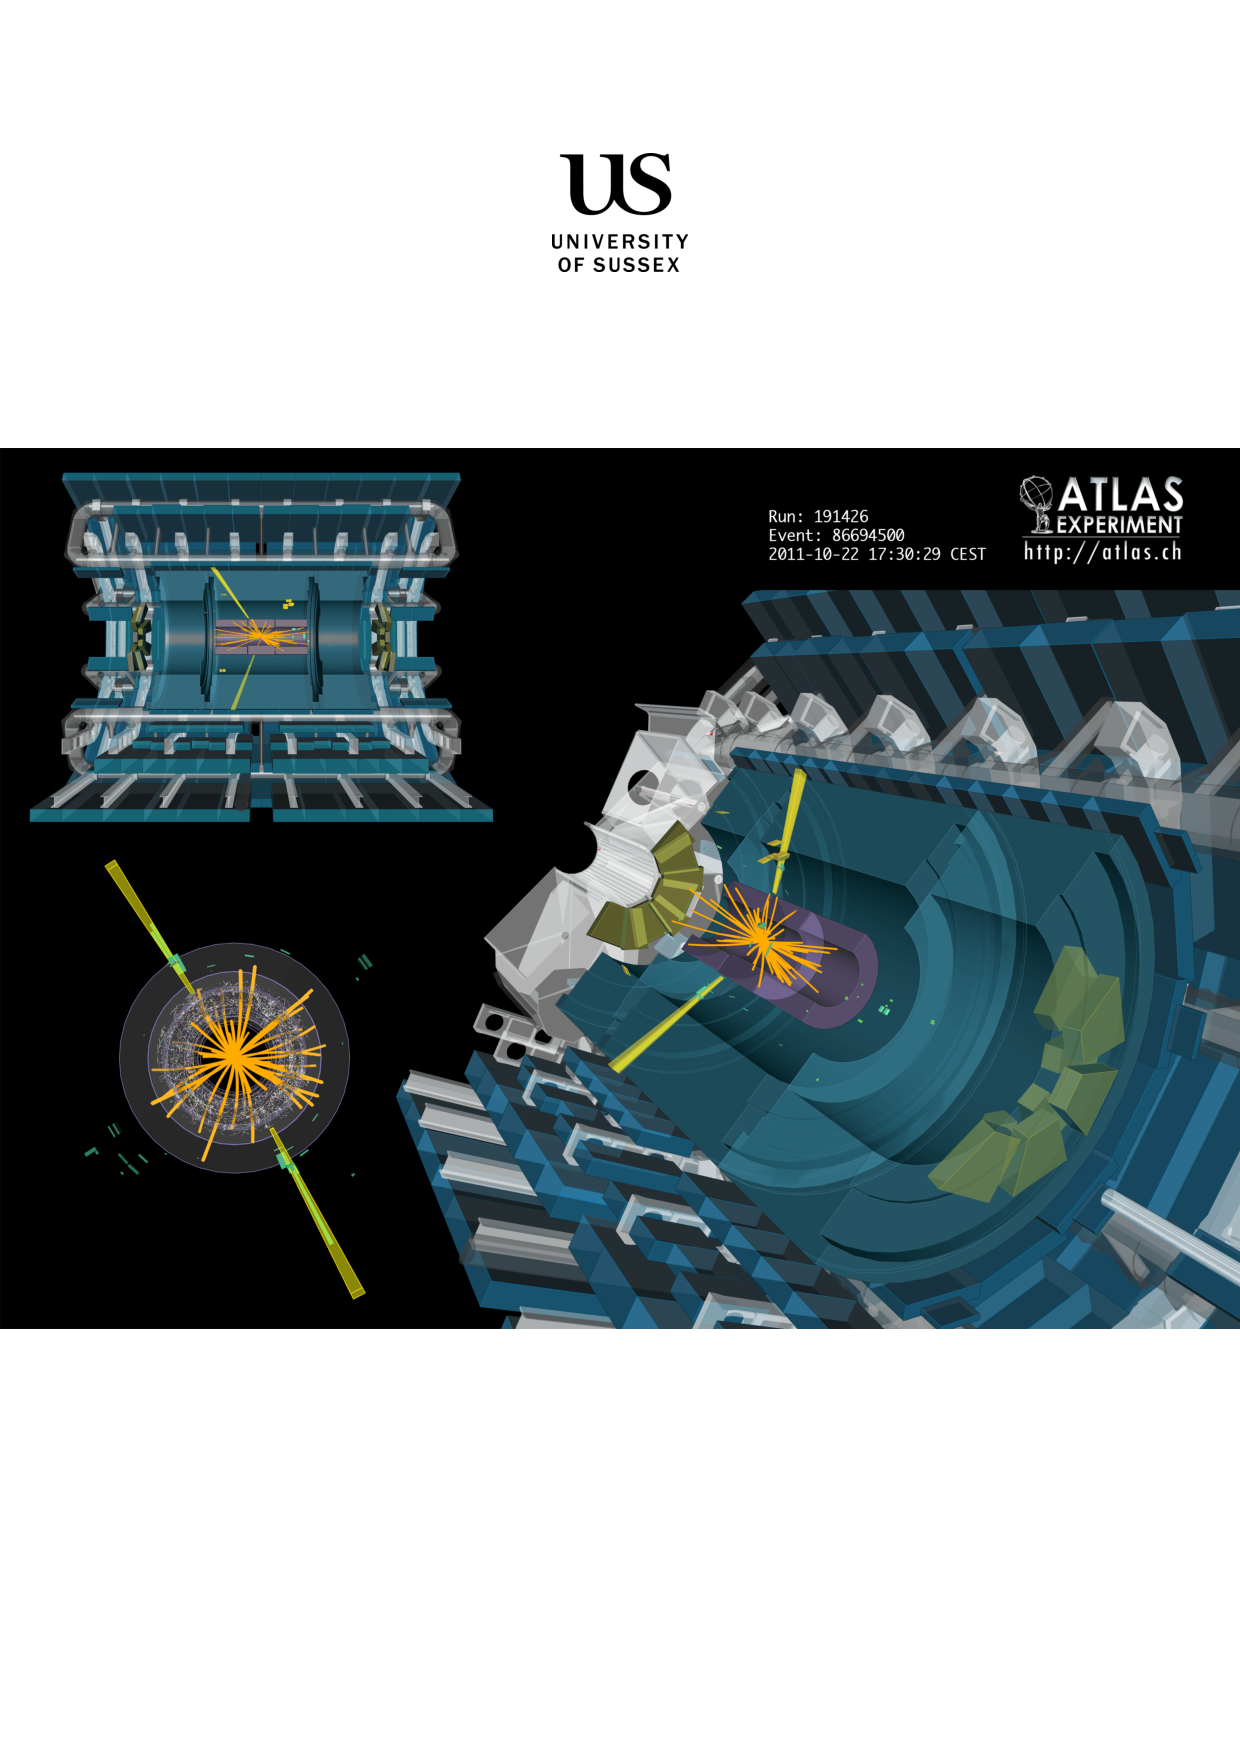
\includegraphics[width=\paperwidth]{cover_picture.pdf}};
\draw (current page.center) node [fill=ocre!30!white,fill opacity=0.6,text opacity=1,inner sep=1cm]{\Huge\centering\bfseries\sffamily\parbox[c][][t]{\paperwidth}{\centering Collider Physics using ATLAS Open Data\\[15pt] % Book title
{\Large Advanced Physics Laboratory}\\[5pt] % Subtitle
{\large Version: 1.1 \ \ \ \ Contact: I.Vivarelli@sussex.ac.uk}\\[20pt] % Subtitle
{\huge Physics and Astronomy Department}}}; % Author name
\end{tikzpicture}
\vfill
\endgroup

%\clearpage
%
%\tableofcontents
%
%\newpage
%
%\section{Introduction} 
%% !TEX root = ../main.tex

This Advanced Physics Laboratory experience will guide you through the main steps that a physicist working in a large particle physics collaboration (like ATLAS, CMS, but also DUNE, NOVA, etc.) has to to do look at the experiment data and draw conclusions about the underlying physics. Specifically, you will be using simulated and real ATLAS proton-proton collisions at $\sqrt{s} = 13\ \TeV$ to do a series of particle physics measurements. Given the structure of the course you are following with us, your particle physics knowledge at the time of this experience will be limited: the first part of this document is a very quick and dirty introduction to the particle physics you need to know to be able to understand what you are doing when running the experiments. You will also need a review (or introduction, depending on previous experience) to some software tools that will be useful for this experience, but also for your future career, so long as it involves any software development and data analysis. 
%
%\section{Objectives}
%\label{sec:objectives} 
%% !TEX root = ../main.tex

The main aim of the experience connected with this handbook is to get a glimpse of frontier particle physics. You will be \textit{seeing} the basic bricks with which our universe is composed. You will be observing $Higgs$ bosons, and top quarks and $W$ and $Z$ bosons. These particles form the foundations of our understanding of the electroweak interaction, mass, and stability of our universe. You will be asked to verify some of the properties of these particles, and hopefully by the end fo the experience you will have a better understanding of the work that collider physicists do. 

This is what you are expected to do and prepare: 

\begin{itemize}
\item{\textbf{Preparation:}} You should address all exercises labelled as Ex 1...N in sections 3-5. The answers should mostly be available in this same handbook, but they require some thinking and elaboration on your side. you may need to look for other resources on the web and at the library to answer some of the most complex ones. 
\item{\textbf{Experiments:}} You should run the experiments in Section~\ref{sec:experiments}, document what you have done in a logbook (maybe electronic), and answer all questions as quantitatively as possible. The three experiments are in increasing difficulty. 
\end{itemize} 


%
%\clearpage
%
%\section{Particle Physics} 
%\label{sec:particle_physics}
%% !TEX root = ../main_orange.tex


Particle physics is an area of physics that deals with the behaviour of the most basic constituents of matter and their mutual interaction. This section wants to serve as a \textbf{very} compact summary of the main aspects of particle physics that you need to know to be able to run this experiment. The book which is used in the particle physics module here at the University of Sussex is the one listed in Ref.~\cite{shaw}: you may want to have a look there for more details. 

Particles are very small, and, for what concern this experiment, very fast as well. A mathematically sound physical theory of particle physics needs to be compliant with the laws of quantum mechanics and (special) relativity. The standard formulation of particle physics is done in terms of a Quantum Field Theory. We will avoid almost any reference to QFT: this will imply that in some places you will have to ``believe'' some of the results that will be presented. 

Depending of the property one is interested in, particles can be grouped in a few different ways:

\begin{itemize}
\item If one is interested in their spin properties, particles are divided into \textbf{fermions}, whose spin is fractional (like $1/2$, $3/2$, etc.), and \textbf{bosons}, whose spin is integer. All elementary particles that constitute ordinary matter (the up and down quarks, the electrons) are fermions. All particles that mediate an interaction (the photon, the Higgs boson, etc.) are bosons.
\item If one is interested in their spacial size, particles are divided into \textbf{elementary} (more on them later), that should be imagined essentially as a geometrical point in space, with no physical size, and \textbf{composite}, that is, bound states of other particles. Examples of elementary particles are the electron and the quarks. Composite particle examples are the proton and the neutron. 
\item If one is interested in the interactions they feel, particles are divided into \textbf{leptons}, that interact through gravity and the electroweak force, and \textbf{hadrons} which interact through gravity, the electroweak force and the strong nuclear force. The electron and neutrinos are leptons, the quarks are hadrons.
\end{itemize}

Other groupings are possible: we will introduce them if and when they will be needed. In the following, the word ``particle'' will be used with the meaning of ``elementary particle'', unless stated otherwise.

Particles are objects with a mass of the order of that of the proton. There are large variations on this order of magnitude: the heaviest known elementary particle is the top quark, whose mass is about 172 times that of the proton. The electron is the lightest massive particle, with a mass of about half of a thousandth of a proton. Massless particles exist as well (the photon mass is zero, that of the neutrinos is very small although not zero).

\begin{figure}[tb] 
	\centering
	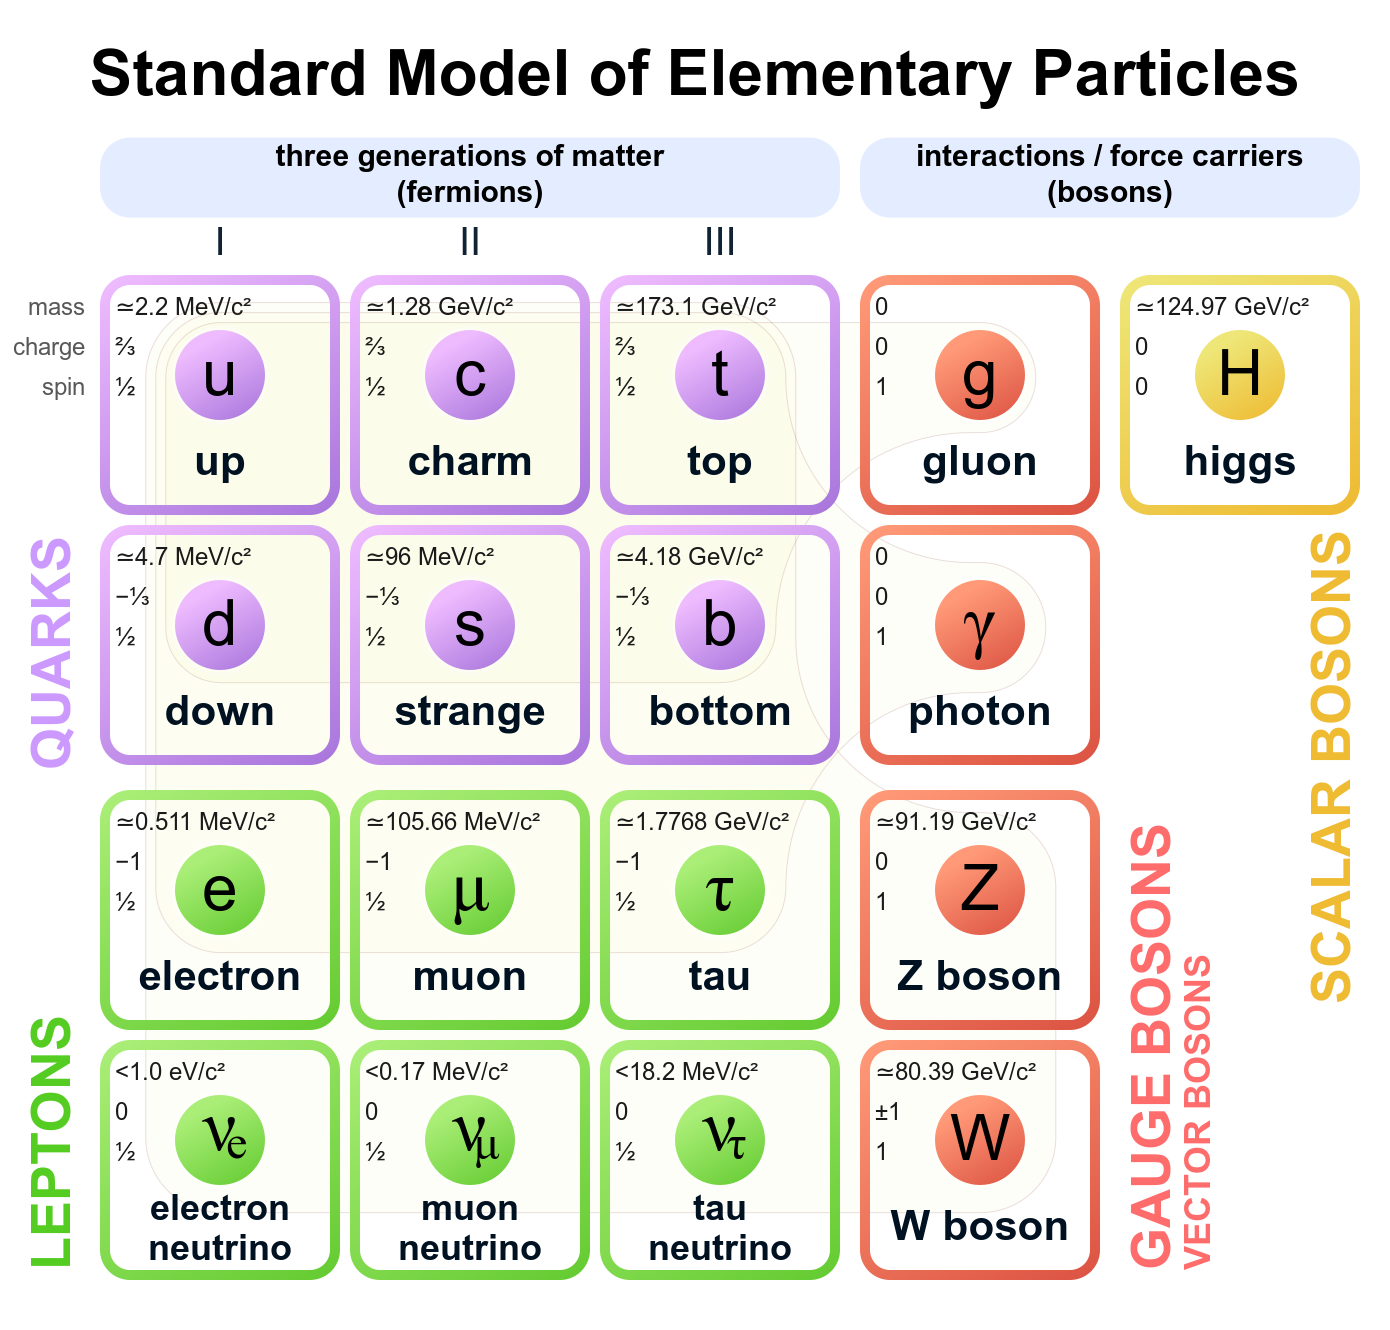
\includegraphics[width=0.5\columnwidth]{Figures/Standard_Model_of_Elementary_Particles.png}
	\caption{Particle content of the Standard Model of Particle Physics. For each particle, the mass, the charge and the spin are reported. Please bear in mind that the mass of light quarks ($u$, $d$, $s$) is not straightforward to define and estimate, given that no free quark can be observed. Taken from Ref.~\cite{SM_wikipedia}.}
		\label{tab:SM}	
\end{figure}


\section{The Standard Model of Particle Physics} 

The best theory of particle physics we have available is the so--called Standard Model of Particle Physics (SM in the following). It specifies the full list of particles, their properties and their interactions. Table~\ref{tab:SM} summarises the particle content of the SM. There are three leptonic families (in green). In each leptonic family, there is a charged lepton and a neutrino of the same flavour. There are also three quark families (in purple). In each quark family there is a quark with charge $+\frac{2}{3}$ and one with charge $-\frac{1}{3}$. Each quark defines its own flavour. Not shown in the table: for each particle family there is an identical family composed by anti-particles. So, for the family composed by the electron and its neutrino, there is a family composed by a positively charged electron (the positron) and an antineutrino, and same for the quarks. 

There are also bosons, that mediate the interactions between the particles in the leptonic and quark families (in red). These are: 
\begin{itemize}
\item The photon, that mediates the electromagnetic interaction between charged particles. 
\item The $W^+, W^{-}$ and $Z$ bosons, which mediate the weak interaction between leptons and between quarks. 
\item The gluons, that mediate the strong nuclear interaction between quarks. 
\end{itemize} 

Finally, the Higgs boson is shown in yellow: it interacts with all particles with an intensity that is proportional to the particle mass. 

We will use a helpful graphical tool to represent interactions between particles. These are the Feynman diagrams. Please bear in mind that we will use them only as a graphical tool, but they are actually a representation of quantitative mathematical expressions that allow to precisely calculate how likely a given process is to occur. In these graphs, we will always represent incoming particles on the left and outgoing particles on the right. 

There are important rules that have to be respected when drawing possible Feynman diagrams:
\begin{enumerate}
\item Electric charge, momentum, energy and angular momentum are always conserved at a vertex.
\item Fermions are represented with arrows. An incoming (in a vertex) fermion is represented with an incoming arrow, while an outgoing fermion is represented with an outgoing arrow. For anti-fermions, rules are reversed: an incoming anti-fermion is represented with an outgoing arrow, while an outgoing anti-fermion is represented with an incoming arrow. See examples in Figure~\ref{fig:feyn_example}. 
\item The total number of leptons has to be conserved. Each lepton contributes to the number of leptons with an additive $+1$, while each anti-lepton with an additive $-1$.
\item Likewise, the total number of quarks has to be conserved. Each quark contributes with an additive $+\frac{1}{3}$, while each anti-quark with an additive $-\frac{1}{3}$.
\item As a consequence of rule 1 for angular momentum, a three-line vertex can only be: two fermions and a boson; three bosons.
\item Gluons interact only with quarks and other gluons. 
\item The $Z$ and $\gamma$ bosons always conserve the flavour. So, $Ze^+e^-$, $Zu\bar{u}$, $\gamma c\bar{c}$ are perfectly legal vertices, $Z e^+ \mu^{-}$, $Zc\bar{s}$ and $\gamma e^-\mu^+$ are not.
\item The $Z$ boson does not interact with the photon.
\item The $W$ boson interaction conserves the leptonic flavour. So $We\bar{\nu}_e$ is a legal vertex, but $We\bar{\nu}_{\mu}$ is not. 
\end{enumerate}

Figure~\ref{fig:feyn_example}~\footnote{In this handbook, we will always deal with so-called \textit{leading-order} Feynman diagrams. If you want to know more about \textit{higher order} Feynman diagrams, please consult Ref.~\cite{shaw}. We will also neglect possible leading order Feynman diagram vertices that include more than three lines.} shows examples of allowed Feynman diagrams, while Figure~\ref{fig:forbidden_feyn} shows some processes which are not allowed. 

 \begin{figure}[!h]
\begin{center}
\subfigure[Production of a Z boson decaying into a $\mu\bar{\mu}$ pair at an electron-positron collider.]{
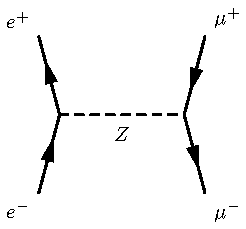
\includegraphics[width=0.2\textwidth]{./Figures/ee_to_Zmumu.eps}
}
\hfill
\subfigure[A diagram for $W$ production at a hadron collider, followed by the $W$ decay into two quarks.]{
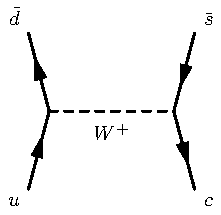
\includegraphics[width=0.2\textwidth]{./Figures/ud_to_Wcs.eps}
}
\hfill
\subfigure[A diagram for $t\bar{t}$ production at a hadron collider.]{
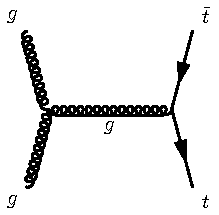
\includegraphics[width=0.2\textwidth]{./Figures/gg_to_ttbar.eps}
}
\hfill
\subfigure[Higgs boson production via the so-called gluon fusion process, followed by $H\rightarrow\gamma\gamma$, at a hadron collider. Both the gluons and the photons are massless particles, the Higgs boson couples to them through intermediate particles.]{
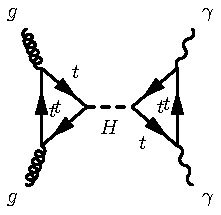
\includegraphics[width=0.2\textwidth]{./Figures/Higgs_gluonFusion.eps}
}
\end{center}
\caption{Examples of valid Feynman diagrams. For each of them, the fermion lines do not stop within the diagram, rather they enter and exit the diagram fully. This is a consequence of angular momentum and charge conservation.}
\label{fig:feyn_example}
\end{figure}

 \begin{figure}[!h]
\begin{center}
\subfigure[Violation of charge conservation at the $W$ production vertex.]{
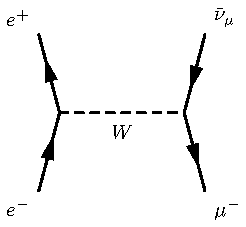
\includegraphics[width=0.2\textwidth]{./Figures/ee_to_Wmumu.eps}
}
\hfill
\subfigure[Flavour violation at the $Z$ decay vertex. The $Z$ boson only couples to leptons and quarks of the same flavour.]{
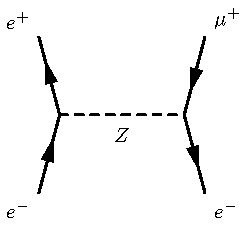
\includegraphics[width=0.2\textwidth]{./Figures/ee_to_Zemu.eps}
}
\hfill
\subfigure[Charge conservation violation at the Higgs boson production vertex.]{
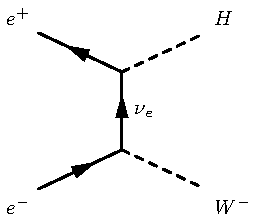
\includegraphics[width=0.2\textwidth]{./Figures/ee_to_WH.eps}
}
\hfill
\subfigure[Four-fermion interaction vertices do not exist in the Standard Model.]{
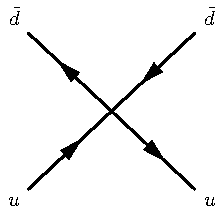
\includegraphics[width=0.2\textwidth]{./Figures/ud_to_ud.eps}
}
\hfill
\subfigure[There is a broken fermion line at both vertices (violation of charge, angular momentum, baryon number conservation).]{
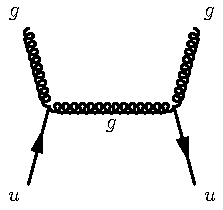
\includegraphics[width=0.2\textwidth]{./Figures/ug_to_g.eps}
}
\hspace{1cm}
\subfigure[The Higgs boson does not couple directly with particles with no mass.]{
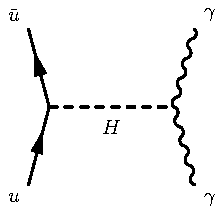
\includegraphics[width=0.2\textwidth]{./Figures/uu_to_Hgamgam.eps}
}
\end{center}
\caption{Examples of processes which are {\color{red} NOT} allowed in the Standard Model, with a quick explanation of why they are not allowed.}
\label{fig:forbidden_feyn}
\end{figure}



\section{Special relativity and units}

In particle physics it is customary to choose a system of units in which the value of the Planck constant $\hbar$ and the speed of light $c$ are both set to unity: $\hbar = c = 1$. Energy and momentum are therefore measured with the same units. Often the electronvolt (eV) is the energy unit chosen. For the applications of this experiment, we will be using MeV, GeV and TeV. Because of the Heisenberg uncertainty principle, the unit for space is also fixed: 

\begin{align}
\Delta p \Delta x \sim \hbar = 1 \implies [x] = \frac{1}{[p]}  = \frac{1}{\mathrm{MeV}}
\end{align}

Likewise, from $\Delta E \Delta t \sim \hbar = 1$, it follows that time has the same units of space. From $E=mc^2$, it follows that mass and energy have the same units. 


The particle free motion is described in terms of their energy $E$ and momentum $\mathbf{p}$. The three momentum components and the energy form a so-called 4-vector. You already have the knowledge of what a 4-vector is, but probably nobody has used this name just yet. Let's start from a standard position vector in space $\mathbf{x}$, with components $(x,y,z)$ in a given reference frame $S$. Let's name this a 3-vector (and you can probably already guess where I am going...). You know well that in special relatively the spacial coordinates and the time of a given event cannot be treated independently from each other, simply because they mix if one describes the same event from a different reference frame in uniform motion with respect to the original one.  For a change of reference frame from a frame $S$ to one $S'$ moving with speed $v$ along $\hat{x}$ with respect to $S$, the 4-vector transforms into $(\mathbf{x'},t')$ such that:

\begin{align}
x' &= \gamma \left(x + \beta t\right) \nonumber \\
y' &= y \nonumber \\
z' &= z \nonumber\\
t' &= \gamma \left(t + \beta x\right)
\end{align}
\label{eq:lorentz_transform}

\noindent where we are using units in which the speed of light $c$ is equal to 1. $x'$ is a function of both $x$ and $t$, and the same is true for $t'$.  Perfect! Let's then define a 4-vector as $x_\mu = (x,y,z,t)$. The components of a 4-vector transform by Lorentz boost as in Eq.~\ref{eq:lorentz_transform}.

The symbols $\gamma$ and $\beta$ are defined (for $c=1$) by: 

\begin{align}
\gamma = \frac{1}{\sqrt{1-v^2}} \qquad \beta = \frac{v}{c} = v
\end{align}

The transformations in Eq.~\ref{eq:lorentz_transform} are such that the product  

\begin{align}
s = t^2 - \mathbf{x} \cdot \mathbf{x}
\end{align}

\noindent is invariant for Lorentz transformations, that is, its value is the same in the reference frame $S$ or in any other boosted frame $S'$. 

\begin{exercise}
Prove it! Prove that  $t^2 - \mathbf{x} \cdot \mathbf{x} =  t'^2 - \mathbf{x'} \cdot \mathbf{x'}$, where the primed quantities are connected to the non-primed ones by a Lorentz transformation like in eq.~\ref{eq:lorentz_transform}
\end{exercise}

So, momentum and energy form another 4-vector, $p_{\mu} = (p_x,p_y,p_z,E)$. That means that if I go from one reference frame to another in relative motion along $\hat{x}$,

\begin{align}
p_x' &= \gamma \left(p_x + \beta E\right) \nonumber \\
p_y' &= p_y \nonumber \\
p_z' &= p_z \nonumber\\
E' &= \gamma \left(E + \beta p_x\right)
\end{align}
\label{eq:lorentz_transform_momentum}

It also means that $E^2 - \mathbf{p}\cdot \mathbf{p}$ is an invariant.......

\subsection{Invariant Mass}
\label{sec:invariant_mass}

The fact that for a 4-vector of type $\left(\mathbf{m}_x, m_t\right)$ the product $s_{m} = m_t^2 - \mathbf{m}_x \cdot \mathbf{m}_x$ is Lorentz-invariant (that is, it is the same in every reference frame, regardless of its boost) is general. The number $\sqrt{s_{m}} = \sqrt{m_t^2 - \mathbf{m}_x \cdot \mathbf{m}_x}$ is the \textit{magnitude} of the 4-vector. As pointed out earlier, the energy and momentum form a 4-vector $\left(\mathbf{p},E\right)$. Therefore the combination $s = E^2-p^2$ (where $p$ indicates the magnitude of $\mathbf{p}$) is Lorentz-invariant. What is the value of this Lorentz-invariant quantity? Let's consider a particle of mass $m$. In its own rest frame: 

\begin{align} 
E &= m \\ 
\mathbf{p} &= 0 \\ 
s^2 &= E^2 - p^2 = m^2
\end{align}

\noindent But since $s^2$ is Lorentz-invariant, \textit{this mathematical combination of the momentum and the energy of the particle will yield the particle mass regardless of the rest frame where it is computed!}. We will use this fact repeatedly.

\section{Proton-proton Collisions - Collider Physics Variables}
\label{sec:collider_physics_variables}

In this experience, we will study proton-proton collisions produced by the LHC and recorded by ATLAS. The LHC collides two beams of protons head-on. The energy of the protons in each beam is $\ebeam = 6.5\ \TeV$. 

As said earlier, protons are not elementary particles. They are made by three \textit{valence} quarks (two $u$ and one $d$) and a \textit{sea} of other quark-antiquark pairs and gluons, which are created and destroyed continuously according to quantum mechanics. All these particles (the valence quarks and the sea quarks and gluons) take the generic name of \textit{partons}. 

The scale for the proton binding energy is given by its own mass ($\sim 1\ \GeV$). With respect to the typical energy transfer in a LHC collision of interest, with energy exchanged of hundreds of GeV, the binding energy of the proton is small. Therefore the partons in the proton in a LHC collision \textbf{can be considered as free}: the LHC is indeed a parton collider. 

Partons inside a proton however do not have the same energy/momentum as the proton of course: it is the sum of the energies and momenta of all partons that will yield the energy and momentum of the proton. Let's say that each parton $i$ in the collision carries a fraction $x_i$ of the momentum and energy of the proton. The 4-vectors of the protons and colliding partons are (neglecting all masses, and setting the $\hat{z}$ as beam axis) 

\begin{align}
\mathrm{Proton 1}&: \left(0,0,\ebeam,\ebeam\right) \\
\mathrm{Proton 2}&: \left(0,0,-\ebeam,\ebeam\right) \\
\mathrm{Parton 1}&: \left(0,0,x_1\ebeam,x_1\ebeam\right) \\
\mathrm{Parton 2}&: \left(0,0,-x_2\ebeam,x_2\ebeam\right) \\
\end{align}

The magnitude of the 4-vector corresponding to the sum of the two proton 4-vectors is 

\begin{align}
\sqrt{s} = \sqrt{\left(2\ebeam\right)^2 - \left(\ebeam-\ebeam\right)^2} = \sqrt{4\ebeam^2} = 2\ebeam = 13\ \TeV
\end{align}

\noindent which is known as the centre-of-mass energy of the LHC. However, this is \textbf{not} the centre of mass energy of the parton-parton collisions! The actual particles colliding are the partons. Their own centre-of mass energy is:

\begin{align*}
\sqrt{\hat{s}} = \sqrt{\left( x_1 + x_2 \right) ^2 \ebeam^2 - \left( x_1 - x_2\right)^2 \ebeam^2}
\end{align*}

\begin{exercise}
Prove that this implies $\sqrt{\hat{s}} = \sqrt{x_1 x_2} \sqrt{s}$
\end{exercise}

By the way: the frame in which the proton-proton collision happens at rest (the laboratory frame) does not coincide with that in which the parton collision happens at rest. With respect to the laboratory frame, the parton-parton collision happens in a system which is boosted along the beam axis by $p_{\mathrm{boost}} = |x_1-x_2| \ebeam$.

 \begin{figure}[!h]
\begin{center}
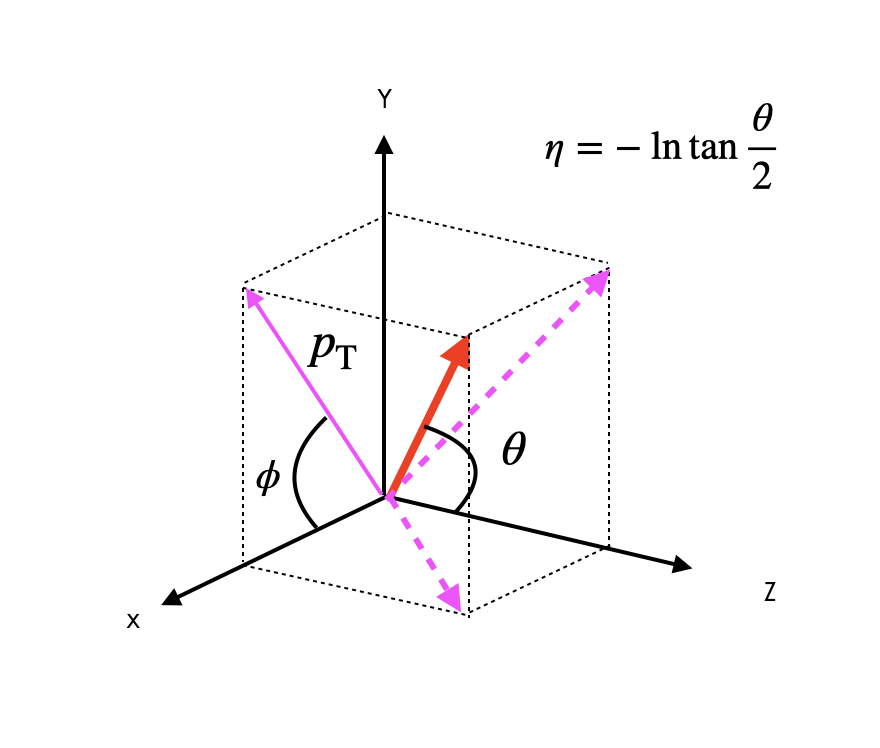
\includegraphics[width=0.5\textwidth]{./Figures/collider_physics_variables.png}
\end{center}
\caption{Diagram of the kinematic variables used at a hadron collider. The $z$ axis coincides with the beam axis.}
\label{fig:collider_variables}
\end{figure}


Let's recap: on an \textbf{event-by-event basis}, the parton-parton collision happens in a frame with a different boost with respect to the laboratory frame, and the collision energy is smaller than the nominal proton-proton centre-of-mass energy. 

\begin{exercise}
The mass of the top quark is 172 GeV. The SppS, a collider colliding protons and antiprotons at CERN, worked up to energies of $\sqrt{s} = 900\ \GeV$. Yet, we had to wait for the Tevatron ($\sqrt{s} = 1.8\ \TeV$) for the top quark discovery. Why?
\end{exercise}

\begin{exercise}
Draw one of the most relevant Feynman diagram for the production of the following particles at the LHC. If quarks are involved, specify if they are likely to be valence or sea quarks: $Z$ boson production, $W$ boson production, $t\bar{t}$ production.
\end{exercise}

\begin{exercise}
The mass of the $W$ boson is $m = 80\ \GeV$. In a given collision pp collision at $\sqrt{s} = 13\ \TeV$, the $W$ boson is produced by a collision of a valence quark with $x = 0.3$,  and a sea quark. Find $x$ of the sea quark and compute $p_{\mathrm{boost}}$ for this collision.
\end{exercise}


So, in practice what happens is that in each event, the LHC experiments look at a collision happening with an unknown boost along the $\hat{z}$ axis. There is one important implication: if we measure any variable which is not Lorentz-invariant, we would make a big confusion when measuring it in many events, because we would mix up values belonging to different reference frames! This implies we have to carefully choose the quantities that we measure at a hadron collider like the LHC to characterise the particles' final states: we should avoid using any variable relying on \textit{longitudinal} quantities, that is, quantities relying on variables measured along the $\hat{z}$ axis. The reason  Therefore, the variables we use at a hadron collider are (see also Figure~\ref{fig:collider_variables}) 

\begin{itemize}
\item The momentum in a plane transverse to the beam, $\pt$.
\item The angle $\phi$ in the transverse plane with respect to the direction pointing towards the LHC centre.
\item The mass.
\end{itemize}

And now we have a problem, because three variables do not determine a 4-vector, of course. We need somewhat to provide the direction with respect to the beam axis. This is done with the rapidity $y$ variable, or with its approximated variable (valid for massless particles) the pseudorapidity $\eta$. 

\begin{align*}
y &= \frac{1}{2} \ln \left(\frac{\mathbf{E} + p_z}{\mathbf{E} + p_z} \right) \\
\eta &= -\ln \tan \frac{\theta}{2}
\end{align*}

\section{Cross-section and luminosity}
\label{sec:cross_section_lumi}

Imagine you have a beam of particles impinging on a slab of targets, and that the targets are small enough that you can neglect shielding effects of one target with respect to another. The total number of interactions that you will observe per unit time will be determined by:

\begin{itemize}
\item characteristics of the beam of particles (how many particles per unit surface per unit time you are shooting, that is, the incoming flux of particles),
\item the target density,
\item the transverse area that the targets offer to the beam, that is, the cross-section of the individual targets. 
\end{itemize}

Inheriting this language, we define the cross-section and the luminosity of a given process at a hadron collider such that the number of occurrences of that process that we observe per unit time is given by: 

\begin{align}
\frac{dN}{dt} = \sigma \times \mathcal{L}
\end{align} 

In the example above, the luminosity is something connected with how many protons per beam we have, how many beams are circling the LHC, etc., while the cross-section is intrinsically connected with the physical interaction yielding a given process. The cross-section units are those of a surface (cm$^2$, for example\footnote{Particle physics cross sections are normally expressed in barns, where $1\ \mathrm{barn} = 10^{-24}\ \mathrm{cm}^2$}), while those of the luminosity are

\begin{align}
[\mathcal{L}] =  [\mathrm{surface}]^{-1}\cdot [\mathrm{time}]^{-1}.
\end{align}

A typical number $\mathcal{L}$ during the LHC Run 2 is $\mathcal{L} \sim 2\times 10^{34}$ cm$^{-2}$ s$^{-1}$. The total number of events we will count for a given process in a given period of time is of course given by 

\begin{align}
N = \int_{\Delta T} \frac{dN}{dt} dt = \int_{\Delta T} \sigma \times \mathcal{L} dt &= \sigma \int_{\Delta T} \mathcal{L} dt = \sigma \Lint, \\ 
\Lint &= \int_{\Delta T} \mathcal{L} dt.
\end{align}

The data collected by a given experiment over a period of time are typically expressed with the corresponding \textit{integrated luminosity} $\Lint$. Let's make an example. The ATLAS experiment has collected a number of proton-proton collisions corresponding to $\Lint = 139\ \ifb$ during the so-called Run 2 at $\sqrt{s} = 13\ \TeV$. The production cross-section for top pairs is predicted to be $\sigma_{t\bar{t}} = 831\ \mathrm{pb}$. Let's compute how many top pair production events we expect to have collected during the full Run 2: 

\begin{align}
N_{t\bar{t}} = \sigma_{t\bar{t}} \times \Lint &= 831 \times 10^{-12} \ \mathrm{barns} \times 139 \times \left(10^{-15}\ \mathrm{barns}\right)^{-1} \\
N_{t\bar{t}} &= 1.16\times 10^{8}
\end{align}

So, we expect something like 116 million top pairs to have been produced during Run 2 in ATLAS. 

\begin{figure}[tb] 
	\begin{center}
	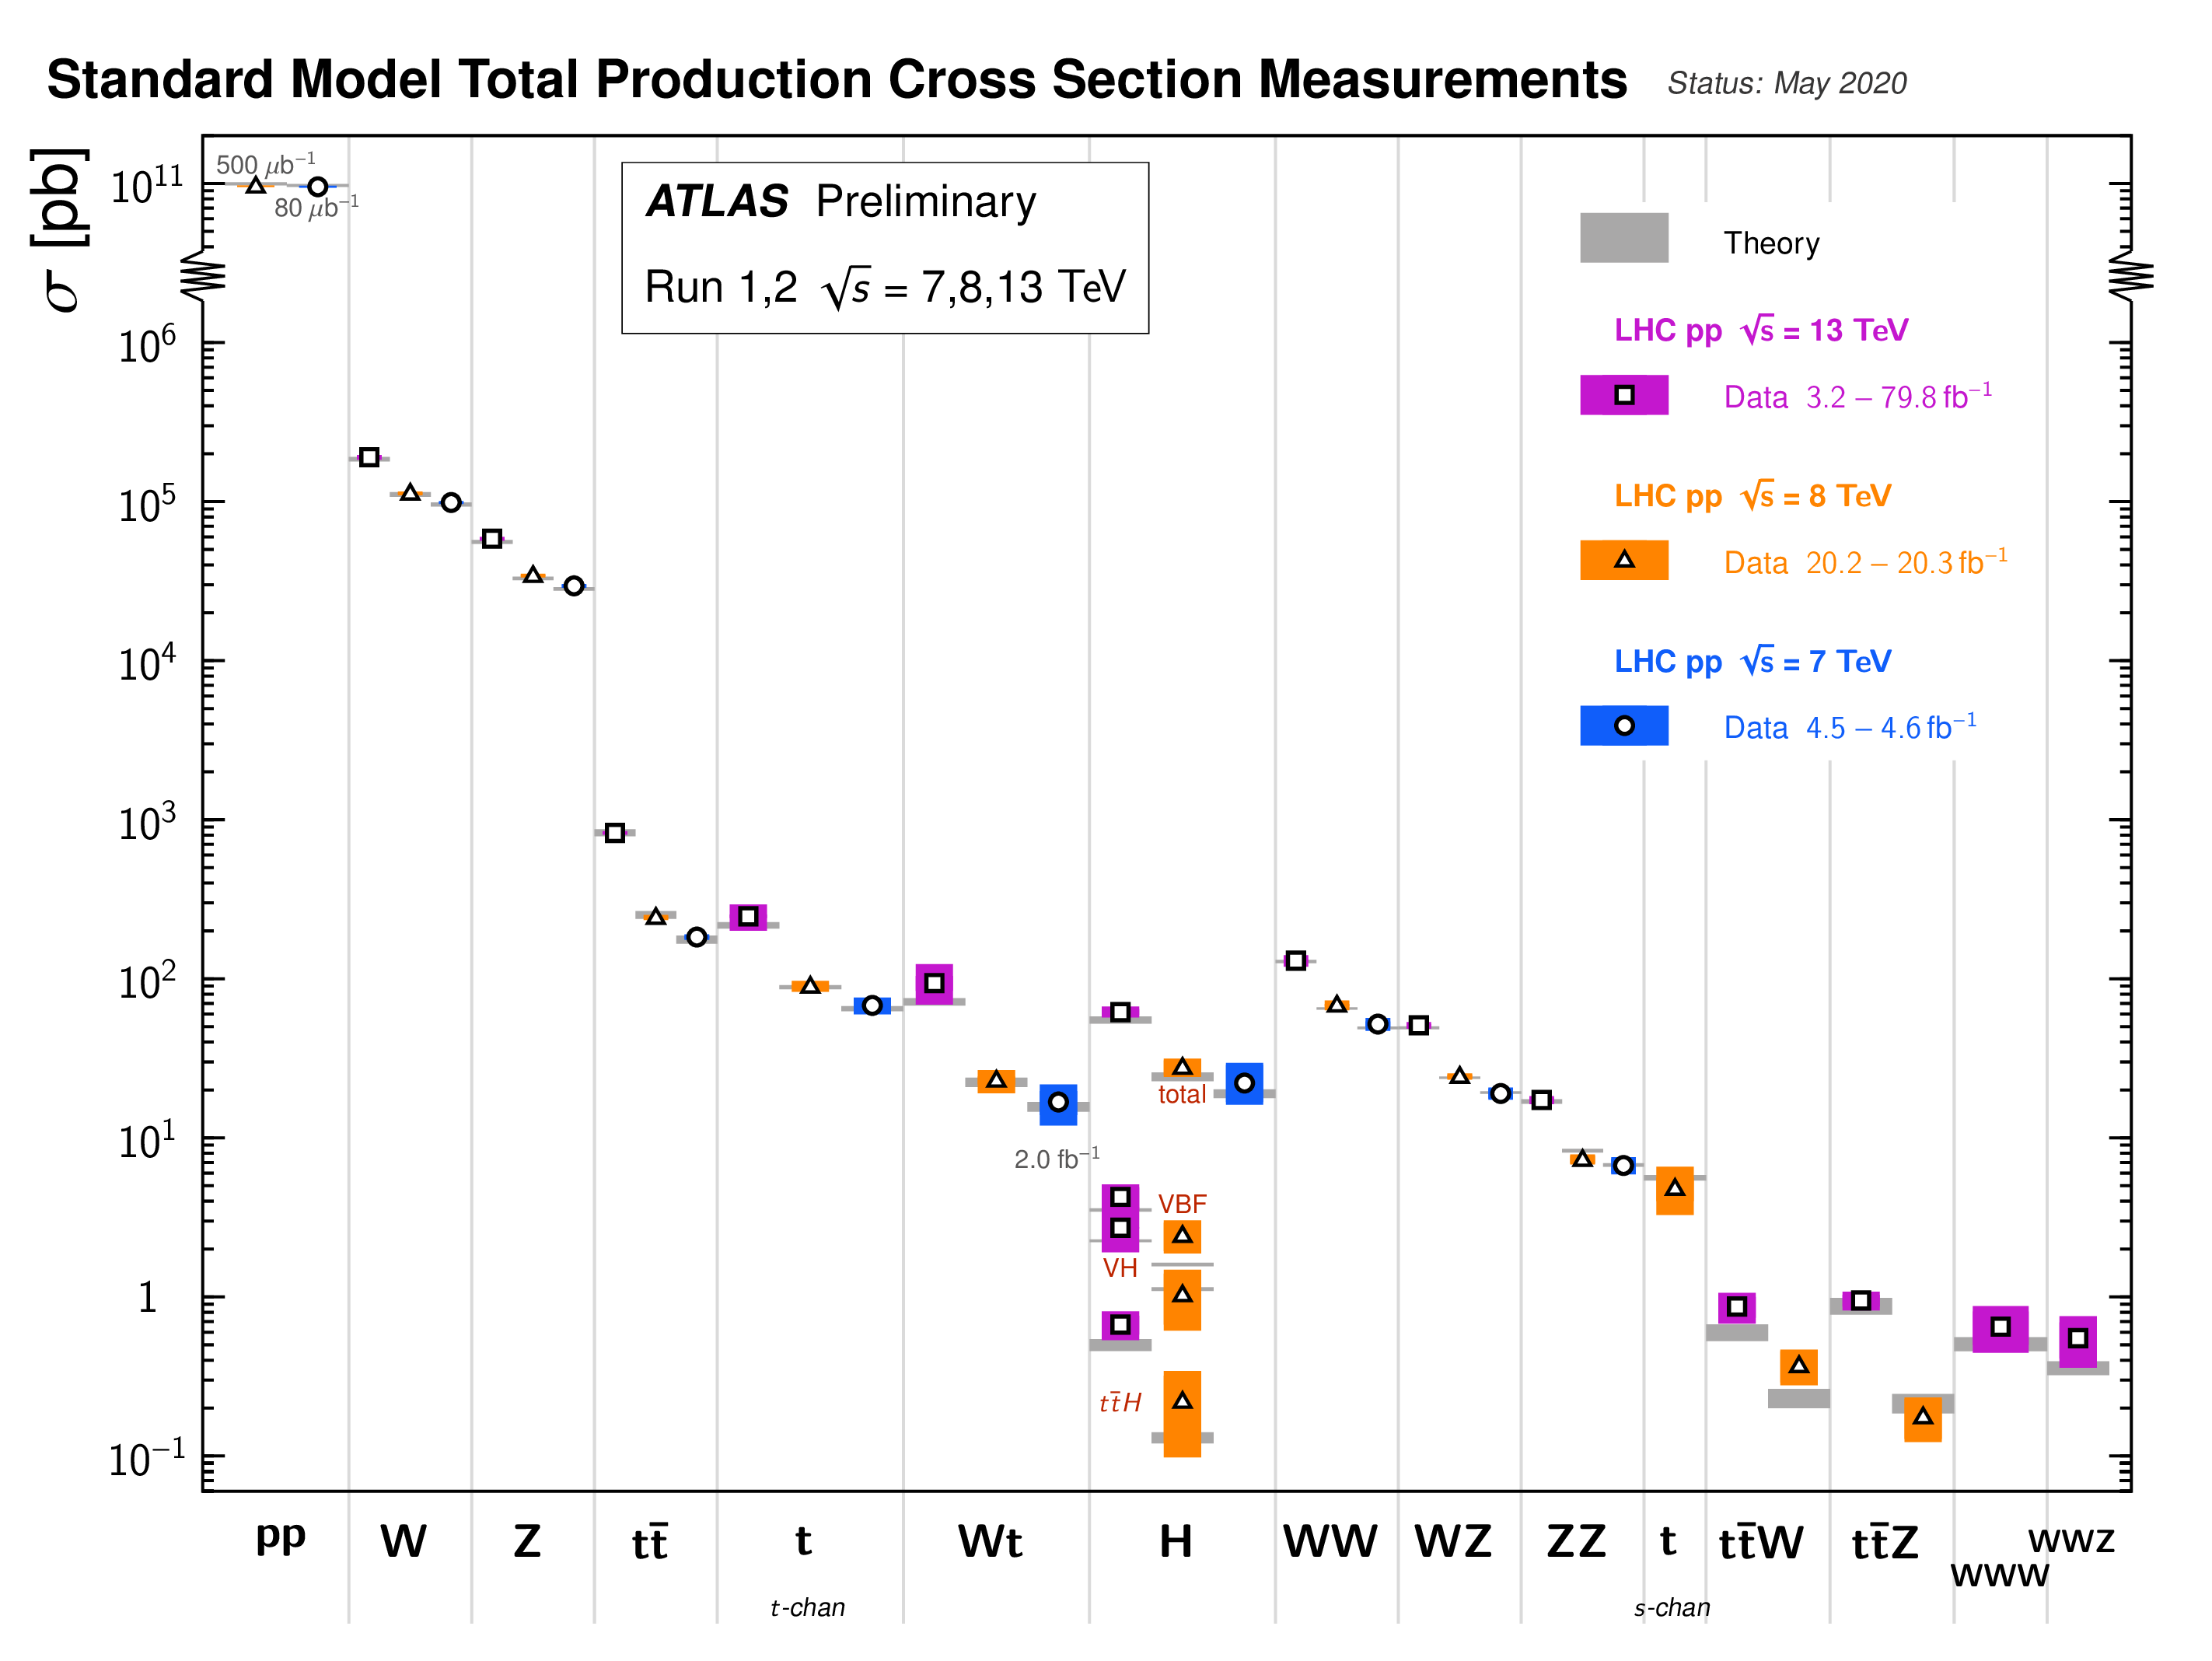
\includegraphics[width=0.7\columnwidth]{Figures/SM_summary.png}
	\end{center}
	\caption{Predictions and ATLAS measurements for the production cross sections of several Standard Model processes. Taken from Ref.~\cite{SM_summary}.}
	\label{fig:SM_summary_plot}
\end{figure}

Now, let's take a close look at Figure~\ref{fig:SM_summary_plot}. It shows the cross-sections for several SM processes at the LHC, for different proton-proton centre-of-mass energies. The proton-proton inelastic cross-section at $\sqrt{s} = 13\ \TeV$ is about $80$ mb. Let's consider one random process as an example, say $WW$ production. The plot tells us that the production cross section is between 100 and 200 pb - let's take 160 pb. So, from the ratio of these numbers, we learn that only one in 500,000 proton-proton collisions will produce $WW$. 

\begin{exercise}
From Figure~\ref{fig:SM_summary_plot}, the Higgs boson production cross-section is $\sigma = 80$ pb. Compute how many Higgs bosons LHC has produced during Run 2, and using the typical value for $\mathcal{L}$ given above, compute how many Higgs bosons per minute the LHC is producing when running at that luminosity. 
\end{exercise}

%
%\clearpage
%
%\section{ATLAS}
%\label{sec:ATLAS}
%% !TEX root = ../main_orange.tex

We will now go though the main aspects of how different particles are reconstructed by ATLAS. This discussion will be crucial to understand the variables that are available for this experiment. 

\section{The ATLAS detector}

ATLAS is a general-purpose particle detector operating at a hadron collider. The structure of the detector is sometimes referred to as onion-like, because different layers of detectors are present when going from the collision point outwards. A detailed description of the ATLAS detector and the technologies used for particle detection goes well below the scope of this document: if you are interested please refer to Ref.~\cite{Aad:2008zzm}. What we will do here is to summarise the main principles behind particle detection.

\begin{figure}[tb] 
	\centering
	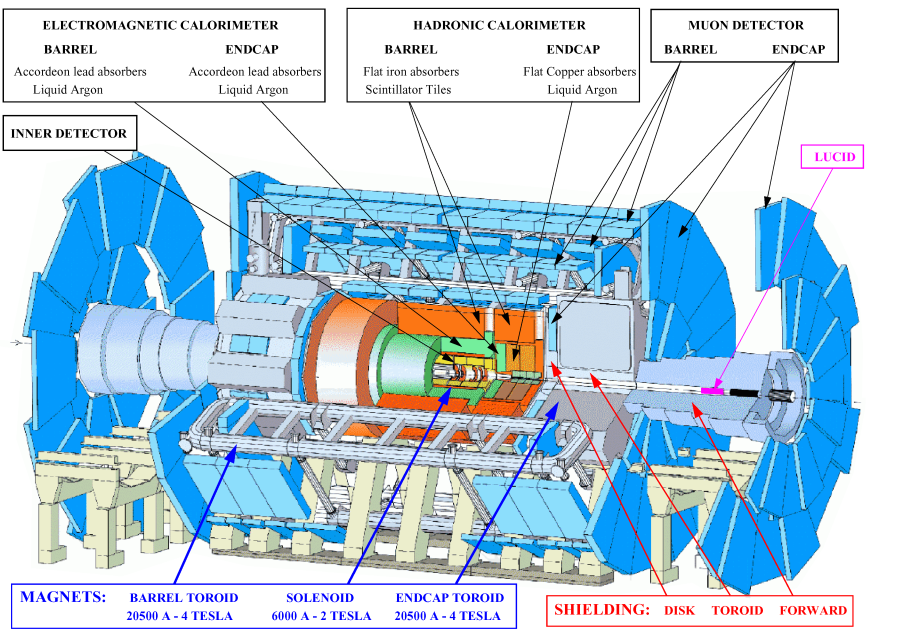
\includegraphics[width=0.7\columnwidth]{Figures/atlas.png}
	\label{fig:ATLAS}
	\caption{Overview of the ATLAS detector. Taken from Ref.~\cite{ATLAS_detector_image}}
\end{figure}

Figure~\ref{fig:ATLAS} shows the various components of ATLAS. Starting from the collision point and going outward: 

\begin{itemize}

\item \textbf{Inner Detector (ID):} Starting at about 3 cm away from the collision point, the inner detector is optimised to measure the position of charged particles. It is immersed in a magnetic field directed along the $z$ axis, such that charged particles trajectories are bent. From the curvature radius it is possible to measure the particle momentum transverse to the magnetic field. 

\begin{exercise}
Remembering that $\mathbf{F} = q \mathbf{v} \times \mathbf{B}$ is acting as centripetal force, estimate the curvature radius of a particle with unit charge and momentum $p = 10\ \GeV$ if $B = 2$~T. 
\end{exercise}

\item \textbf{Electromagnetic (EM) calorimeter:} It stops electrons and photons and measures their energy. It also participate in the energy measurement of hadrons. 
\item \textbf{Hadronic (HAD) calorimeter:} Together with the electromagnetic calorimeter, it measures the energy of neutral and charged hadrons. 
\item \textbf{Muon spectrometer (MS):} Muons and neutrinos are the only particles in the SM that are able to exit the ATLAS calorimeters. The principle of the muon spectrometer is similar to that of the inner detector: the position of muons is measured several times while they are bending in a magnetic field generated by the air-core toroids. From that, a second measurement of the muon momentum is performed, which is typically  combined with the first one taken by the ID. 
\end{itemize}

The subdetectors outlined above are used in combination to reconstruct a number of different final state ``objects''. The number of types of objects which is normally used in an analysis is actually relatively limited. The main features of each of these objects is reviewed below. 

\begin{itemize}
\item{Electrons:} they are identified by a cluster of energy in the EM calorimeter matched with a track in the ID. \textit{Shower shape variables} (that is, the shape of the cluster in the calorimeter), the track quality, and the quality of the matching between the cluster and the track (are the track momentum and cluster energy compatible?) determine the identification. 
\item{Photons:} similar to electrons for the cluster in the EM calorimeter, but with no associated track in the ID. 
\item{Muons:} a track in the MS is almost uniquely identifying a muon (no other charged particle pass through the calorimeters). Typically the MS track is matched to one in the ID. 
\item{Jets:} Quarks and gluons cannot emerge from a collision as such. They go through a process of fragmentation and hadronisation~\cite{fragment_hadronise}, resulting in a jet of collimated hadrons, whose total momentum and direction resembles that of the originating quark/gluon. Such jets are reconstructed mainly from the HAD and EM calorimeter information, but they use some information from the ID as well. 
\item{$b$-jets:} $b$-quarks have a longer lifetime than the other quarks. They travel of the order of a cm or less before decaying. The presence of such secondary vertex (that is, a vertex that does not coincide with the primary one from the pp collision in the transverse plane) can be exploited to ``tag'' the jet as originating from a $b$.
\item{$\tau$ leptons:} The lifetime of the $\tau$ is extremely short. For all practical purposes, it decays before producing any visible effect in the detector. There are two main categories of $\tau$ decays: the leptonic ones and the hadronic ones. If a $\tau$ decays to an electron and muon (through $\tau\rightarrow \ell \bar{nu}_{\ell} \nu_{\tau}$ to conserve the lepton number and flavour), it will be seen as a lepton in the detector. If instead a tau decays to hadrons, then it looks like a very narrow jet with few tracks attached, and it can be identified based on these characteristics. 
\item{Invisible particles:} If an invisible particle is produced (neutrinos, in the standard model), their presence is inferred from the measurement of the total momentum transverse to the beam. Given that the momentum in the plane transverse to the beam is zero before the proton-proton collision, it has to be zero after the collision. The negative vectorial sum of the transverse momenta of all object in the events is called the \textit{missing transverse momentum}, and is an estimate of the total transverse momentum of invisible particles.   
\end{itemize}

Figure~\ref{fig:ttbar_eventdisplay} shows a candidate event for $t\bar{t} \rightarrow \mu \nu_{\mu} + 4\ \mathrm{jets}$. See the caption for further details. 

\begin{figure}[tb] 
	\centering
	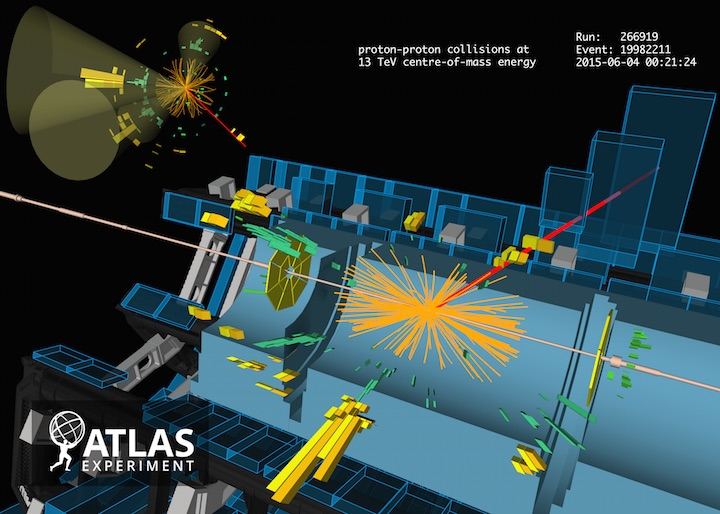
\includegraphics[width=0.7\columnwidth]{Figures/ATLAS_ttbar_candidate_13TeV_VP1_run266919_evt19982211_thumb.jpg}
	\label{fig:ttbar_eventdisplay}
	\caption{Display of a $t\bar{t}$ candidate event from proton-proton collisions recorded by ATLAS at a collision energy of 13 TeV. The red line shows the path of a muon with transverse momentum around 35 GeV through the detector. The green and yellow bars indicate energy deposits in the EM and HAD. From close-by deposits in these calorimeters, four jets are identified with transverse momenta between 25 and 80 GeV. Taken from Ref.~\cite{ATLAS_ttbar_evtdisplay}}
\end{figure}

\section{Monte Carlo and real events}

In this experiment you will deal with two types of events: simulated and real ones. The simulated ones are often referred to as Monte Carlo, or simply MC, events. MC events are the result of a computer simulation, that emulates at best the theory we have for the proton-proton collision. They simulate a specific process (like $Z$ production, or $H$ production), they save the so called truth-level information (that is, the particles that were produced in the collision and that enter the detector) and they also simulate the response of the detector (reco-level). The MC represents our theoretical prediction. 

%It is probably worth at this stage to introduce the concept of cross-section weight. Suppose that I simulate $N$ events of a process whose cross-section is $\sigma$. I know that the data I will be looking at correspond to an integrated luminosity $L$. If I want 


%
%
%\clearpage
%
%\section{Open data: practical guide}
%\label{sec:open_data}
%% !TEX root = ../main.tex

The ATLAS open data consist in a set of MC and real events that the ATLAS collaboration has released for open use. The main web page where they are introduced is \url{http://atlas.cern/resources/opendata}. Please spend some time on this page, explore it, play with it.

The next step is to actually do something. In the ``Online Open Data Analysis'' section of the page, click on ``Analyse ATLAS Open Data with Jupyter Notebooks'', and then in the jupyter-looking window select ``13-TeV-examples'', then "uproot\_python". You should get to this \href{https://notebooks.gesis.org/binder/jupyter/user/atlas-outreach--ection-opendata-hbw4boy5/notebooks/13-TeV-examples/uproot_python}{page}. 

Each notebook corresponds to a different analysis. Please open \verb|HZZAnalysis.ipynb|.
%
%\clearpage
%
%\section{Experiments}
%\label{sec:experiments}
%% !TEX root = ../main.tex



\subsection{Experiment 1: Understanding $H\rightarrow 4\ell$}

In this experiment we will dig deeper into the $H\rightarrow ZZ$ analysis that we have seen earlier. Please document everything you do, including the answers to the questions below, in your logbook. It is suggested you make a copy of the HZZAnalysis.py before you start to modify it.

\begin{enumerate} 
\item Edit the file to print the histogram integrals of the different processes: $ZZ\rightarrow 4\ell$ (red histogram), $Z$ and $\ttbar$ production (shown together in purple), $H\rightarrow ZZ$ (cyan), and, finally, the data. From the discussion about MC weights in Section~\ref{sec:review_notebook}, it should be clear that the integral of the histograms and the actual number of events are different for MC (because of all the applied weights), while they will coincide for the data. 
\item Validate these printouts: try to have a rough estimate of those integrals by looking at the output histogram of the code. Make sure that the rough estimate and the exact printouts are in the same ballpark.
\item Compute the total expected background $B$ by summing the integrals of the $ZZ$, $Z$ and $\ttbar$ processes. We will now compute its agreement with the observed data yield $O$: 
\end{enumerate}

\begin{mybox}
\begin{itemize} 
\item The total background $B$ represents the number of events that one \textit{expects}. Suppose I expect 100 events: the outcome of the actual experiment in general will not be exactly 100. \textit{Assuming that the background expectation is correct}, the probability of a given outcome will be described by a Poisson probability function. 
\item Please review the properties of a Poisson probability function. What is the RMS of a Poisson distribution of mean value $\mu$?
\item Evaluate the level of compatibility of your data yield $O$ by computing the probability $p(O \ge B)$ (if $O<B$, define $p = 0.5$). Such probability is known as a $p$-value. What is the p-value? Small values of the $p$-value indicate low level of compatibility of the hypothesis tested (in this case that the observed yield comes from an expected background level $B$). 
\item Physicists like to convert $p$-values. This conversion can be done for example using \href{https://planetcalc.com/7803/}{this web site}. A high $z$ score, or significance, corresponds to a low level  compatibility of the hypothesis tested (in this case that the observed yield comes from an expected background level $B$). What is the significance in this case?
\end{itemize}
\end{mybox}

\begin{enumerate}[resume]
\item Repeat the points above, but this time compute the background and the observation only in the invariant mass range $120\ \GeV < m_{4\ell} < 130\ \GeV$. What are the p-values and the significance now? 
\item Assume that the difference between the background and observation in the range  $120\ \GeV < m_{4\ell} < 130\ \GeV$ is now a yield due to $H \rightarrow 4\ell$. Knowing that the fraction of Higgs boson production that you select with this analysis is $\epsilon = 2 \times 10^{-5}$ (coming from $BR(H\rightarrow ZZ)=2.6\times 10^{-2}$, $BR(Z\rightarrow \ell\ell) \sim 6\%$, where $\ell = e, \mu$, plus some inefficiency in reconstructing leptons), what is your estimate for the production cross-section of the Higgs boson? Do your best to associate an error to it coming from the number of observed events, and compare to the standard model best prediction of $\sigma(H) = 55$ pb at $\sqrt{s} = 13\ \TeV$, with an uncertainty of 5\%. 
\item Assuming your estimate for the signal and background, how much integrated luminosity would you need to declare a $5\sigma$ discovery?
\end{enumerate}

\subsection{Experiment 2: Plot the di-electron and di-muon invariant mass in data}

In this experiment we will try to use data only to plot the di-lepton invariant mass in events with two leptons, and we will se what the meaning of the cuts on isolation on lines 27 and 31 of \verb|HZZCuts.py| actually do. Finally, we will try to understand the mass resolution for the measurement of $Z\rightarrow e^+e^-$ and $Z\rightarrow \mu^+\mu^-$. We will start from a copy of \verb|HZZAnalysis.py| and associated modules and heavily modify them. To start with, copy \verb|HZZAnalysis.py|, \verb|HZZCuts.py|, \verb|HZZHistograms.py|, \verb|HZZSamples.py|, into new files \verb|ZeeAnalysis.py|, \verb|ZeeCuts.py|, etc. 

\begin{mybox}
\textbf{TIP:} When modifying and playing with the code, reduce \verb|fraction| to something like 0.1 or even lower, to speed up the code while debugging.
\end{mybox}


\begin{enumerate} 
\item Edit the ntuple path to point to the 2lep events rather than the 4lep ones. 
\item Change the Histograms to show only one variable, $m_{ee}$ and plot it from 0\ \GeV to 200\ \GeV in log scale. 
\item Change the cuts file to have only one cut, where you reject events if the leading two leptons are not electrons of opposite charge. 
\item Change the samples to have only the data ones. 
\item Adapt the plotting code to plot only the data. 
\item Add a variable to the DataFrame ($m_{ee}$), similar to what was done with $m_{4\ell}$ in the \verb|HZZAnalysis.py| example.
\item Plot the $m_{ee}$. 
\end{enumerate}

\begin{mybox}
The histogram should display a peak at about 90 GeV, with a lot of events at different masses. The peak at 90 GeV is clearly due to $Z\rightarrow e^+ e^-$, but.... what are all other events?
\end{mybox}

\begin{enumerate} [resume]
\item  Try to add cuts that select on the lepton isolation variables, looking at the examples in  \verb|HZZCuts.py|. What you want is to reject events where either the first or the second leading lepton is not isolated. 
\item Plot again the invariant mass. Comment on differences that you see, especially at small values of $m_{ee}$. 
\end{enumerate}

\begin{mybox}
There are two main categories of leptons that the detector sees: genuine leptons and fake leptons. Genuine leptons are those where reconstruction correctly identifies a lepton as such. Fake leptons are those where the reconstruction thinks there is a lepton, but in fact there wasn't. 

Genuine leptons, in turn, are divided into two categories: prompt leptons arise from an on shell $W$ or $Z$ going to leptons (like in $pp\rightarrow Z\rightarrow e^+ e^-$, or $\ttbar \rightarrow WWbb \rightarrow \mu \nu_{\mu} jjbb$). These leptons are \textit{isolated}, that is, normally do not have other particles nearby. Non-prompt leptons are emitted in hadrons decay, like $B_0\rightarrow e^-\nu K^+$, and they tend to be non-isolated. Isolation is a powerful variable to reject fake and non-prompt leptons.   
\end{mybox}

\begin{enumerate} [resume]
\item Fit the $Z$ peak in data with a gaussian. Now repeat the analysis selecting muons instead of electrons, and fit the $Z\rightarrow \mu\mu$ peak with a gaussian. Compare the widths of the two gaussians. Which one is larger? Can you try to guess why?  
\end{enumerate}

\subsection{Experiment 3: Understanding the events outside the mass window}

In this experiment we will start from the previous one and understand what the other non-$Z$ events in the di-lepton sample actually are. Let's focus on the sample with two opposite charge electrons in the final state. 

\begin{mybox}
\textbf{TIP:} When modifying and playing with the code, reduce \verb|fraction| to something like 0.1 or even lower, to speed up the code while debugging.
\end{mybox}


\begin{enumerate} 
\item Change the Histograms file to add a missing et plot. The range will need to be something like 0\ \GeV to 300\ \GeV in log scale. 
\item Change the samples list to include \ttbar, and diboson ($WW$, $WZ$ and $ZZ$, with DSID in the range 363356 to 363493 - select those that contain two leptons) production.   
\item Modify the plotting code to include the MC, similarly to what you had for \verb|HZZAnalysis.py|
\item Plot the $m_{ee}$ and $E_{T}^{miss}$.
\item Add a cut to reject events with $m_{ee}$ on the $Z$ peak. Plot again the $E_{T}^{miss}$. 
\item Comment about the results. What are the events which are not $Z$ in this data sample? Why do they tend to have a larger missing transverse momentum than $Z$ events?  Plot the expected composition of the data (what fraction is $Z$, what fraction is the rest) for $ E_{T}^{miss} > X$ as a function of $X$.
\end{enumerate}

\begin{mybox}
\textbf{Bonus task:} DSIDs from 392501 to 392521 contain events from physics processes which are not foreseen by the Standard Model, but by some extension of it. Do you want to try and see whether you will be able to discover new physics using the ATLAS Data? Those new processes are $pp\rightarrow \tilde{\chi}^+_1  \tilde{\chi}^-_1 \rightarrow 2\tilde{\chi}^0_1 2\nu \ell^+\ell'^-$. All you need to know is that the new particle $\tilde{\chi}^0_1$ behaves like a neutrino in the detector, and that $\ell$ and $\ell'$ may be of the same flavour or not. Can you design a selection where events would be mostly populated by these events? 
\end{mybox}



%
%\clearpage
%
%
%\appendix
%\addcontentsline{toc}{section}{APPENDICES}

%%----------------------------------------------------------------------------------------
%%	COPYRIGHT PAGE
%%----------------------------------------------------------------------------------------
%
%\newpage
%~\vfill
%\thispagestyle{empty}
%
%\noindent Copyright \copyright\ 2019 John Smith\\ % Copyright notice
%
%\noindent \textsc{Published by Publisher}\\ % Publisher
%
%\noindent \textsc{book-website.com}\\ % URL
%
%\noindent Licensed under the Creative Commons Attribution-NonCommercial 3.0 Unported License (the ``License''). You may not use this file except in compliance with the License. You may obtain a copy of the License at \url{http://creativecommons.org/licenses/by-nc/3.0}. Unless required by applicable law or agreed to in writing, software distributed under the License is distributed on an \textsc{``as is'' basis, without warranties or conditions of any kind}, either express or implied. See the License for the specific language governing permissions and limitations under the License.\\ % License information, replace this with your own license (if any)
%
%\noindent \textit{First printing, March 2019} % Printing/edition date

%----------------------------------------------------------------------------------------
%	TABLE OF CONTENTS
%----------------------------------------------------------------------------------------

%\usechapterimagefalse % If you don't want to include a chapter image, use this to toggle images off - it can be enabled later with \usechapterimagetrue

\chapterimage{vp1-light_1.png} % Table of contents heading image

\pagestyle{empty} % Disable headers and footers for the following pages

\tableofcontents % Print the table of contents itself

\cleardoublepage % Forces the first chapter to start on an odd page so it's on the right side of the book

\pagestyle{fancy} % Enable headers and footers again

%----------------------------------------------------------------------------------------
%	PART
%----------------------------------------------------------------------------------------

%\part{Part One}

%----------------------------------------------------------------------------------------
%	CHAPTER 1
%----------------------------------------------------------------------------------------

\chapterimage{pngegg.png} % Chapter heading image

\chapter{Introduction}

%\section{Introduction}\index{Introduction}
% !TEX root = ../main.tex

This Advanced Physics Laboratory experience will guide you through the main steps that a physicist working in a large particle physics collaboration (like ATLAS, CMS, but also DUNE, NOVA, etc.) has to to do look at the experiment data and draw conclusions about the underlying physics. Specifically, you will be using simulated and real ATLAS proton-proton collisions at $\sqrt{s} = 13\ \TeV$ to do a series of particle physics measurements. Given the structure of the course you are following with us, your particle physics knowledge at the time of this experience will be limited: the first part of this document is a very quick and dirty introduction to the particle physics you need to know to be able to understand what you are doing when running the experiments. You will also need a review (or introduction, depending on previous experience) to some software tools that will be useful for this experience, but also for your future career, so long as it involves any software development and data analysis. 

\section{Objectives}
\label{sec:objectives} 
% !TEX root = ../main.tex

The main aim of the experience connected with this handbook is to get a glimpse of frontier particle physics. You will be \textit{seeing} the basic bricks with which our universe is composed. You will be observing $Higgs$ bosons, and top quarks and $W$ and $Z$ bosons. These particles form the foundations of our understanding of the electroweak interaction, mass, and stability of our universe. You will be asked to verify some of the properties of these particles, and hopefully by the end fo the experience you will have a better understanding of the work that collider physicists do. 

This is what you are expected to do and prepare: 

\begin{itemize}
\item{\textbf{Preparation:}} You should address all exercises labelled as Ex 1...N in sections 3-5. The answers should mostly be available in this same handbook, but they require some thinking and elaboration on your side. you may need to look for other resources on the web and at the library to answer some of the most complex ones. 
\item{\textbf{Experiments:}} You should run the experiments in Section~\ref{sec:experiments}, document what you have done in a logbook (maybe electronic), and answer all questions as quantitatively as possible. The three experiments are in increasing difficulty. 
\end{itemize} 




\chapter{Particle Physics in a nutshell}
\label{sec:particle_physics}
% !TEX root = ../main_orange.tex


Particle physics is an area of physics that deals with the behaviour of the most basic constituents of matter and their mutual interaction. This section wants to serve as a \textbf{very} compact summary of the main aspects of particle physics that you need to know to be able to run this experiment. The book which is used in the particle physics module here at the University of Sussex is the one listed in Ref.~\cite{shaw}: you may want to have a look there for more details. 

Particles are very small, and, for what concern this experiment, very fast as well. A mathematically sound physical theory of particle physics needs to be compliant with the laws of quantum mechanics and (special) relativity. The standard formulation of particle physics is done in terms of a Quantum Field Theory. We will avoid almost any reference to QFT: this will imply that in some places you will have to ``believe'' some of the results that will be presented. 

Depending of the property one is interested in, particles can be grouped in a few different ways:

\begin{itemize}
\item If one is interested in their spin properties, particles are divided into \textbf{fermions}, whose spin is fractional (like $1/2$, $3/2$, etc.), and \textbf{bosons}, whose spin is integer. All elementary particles that constitute ordinary matter (the up and down quarks, the electrons) are fermions. All particles that mediate an interaction (the photon, the Higgs boson, etc.) are bosons.
\item If one is interested in their spacial size, particles are divided into \textbf{elementary} (more on them later), that should be imagined essentially as a geometrical point in space, with no physical size, and \textbf{composite}, that is, bound states of other particles. Examples of elementary particles are the electron and the quarks. Composite particle examples are the proton and the neutron. 
\item If one is interested in the interactions they feel, particles are divided into \textbf{leptons}, that interact through gravity and the electroweak force, and \textbf{hadrons} which interact through gravity, the electroweak force and the strong nuclear force. The electron and neutrinos are leptons, the quarks are hadrons.
\end{itemize}

Other groupings are possible: we will introduce them if and when they will be needed. In the following, the word ``particle'' will be used with the meaning of ``elementary particle'', unless stated otherwise.

Particles are objects with a mass of the order of that of the proton. There are large variations on this order of magnitude: the heaviest known elementary particle is the top quark, whose mass is about 172 times that of the proton. The electron is the lightest massive particle, with a mass of about half of a thousandth of a proton. Massless particles exist as well (the photon mass is zero, that of the neutrinos is very small although not zero).

\begin{figure}[tb] 
	\centering
	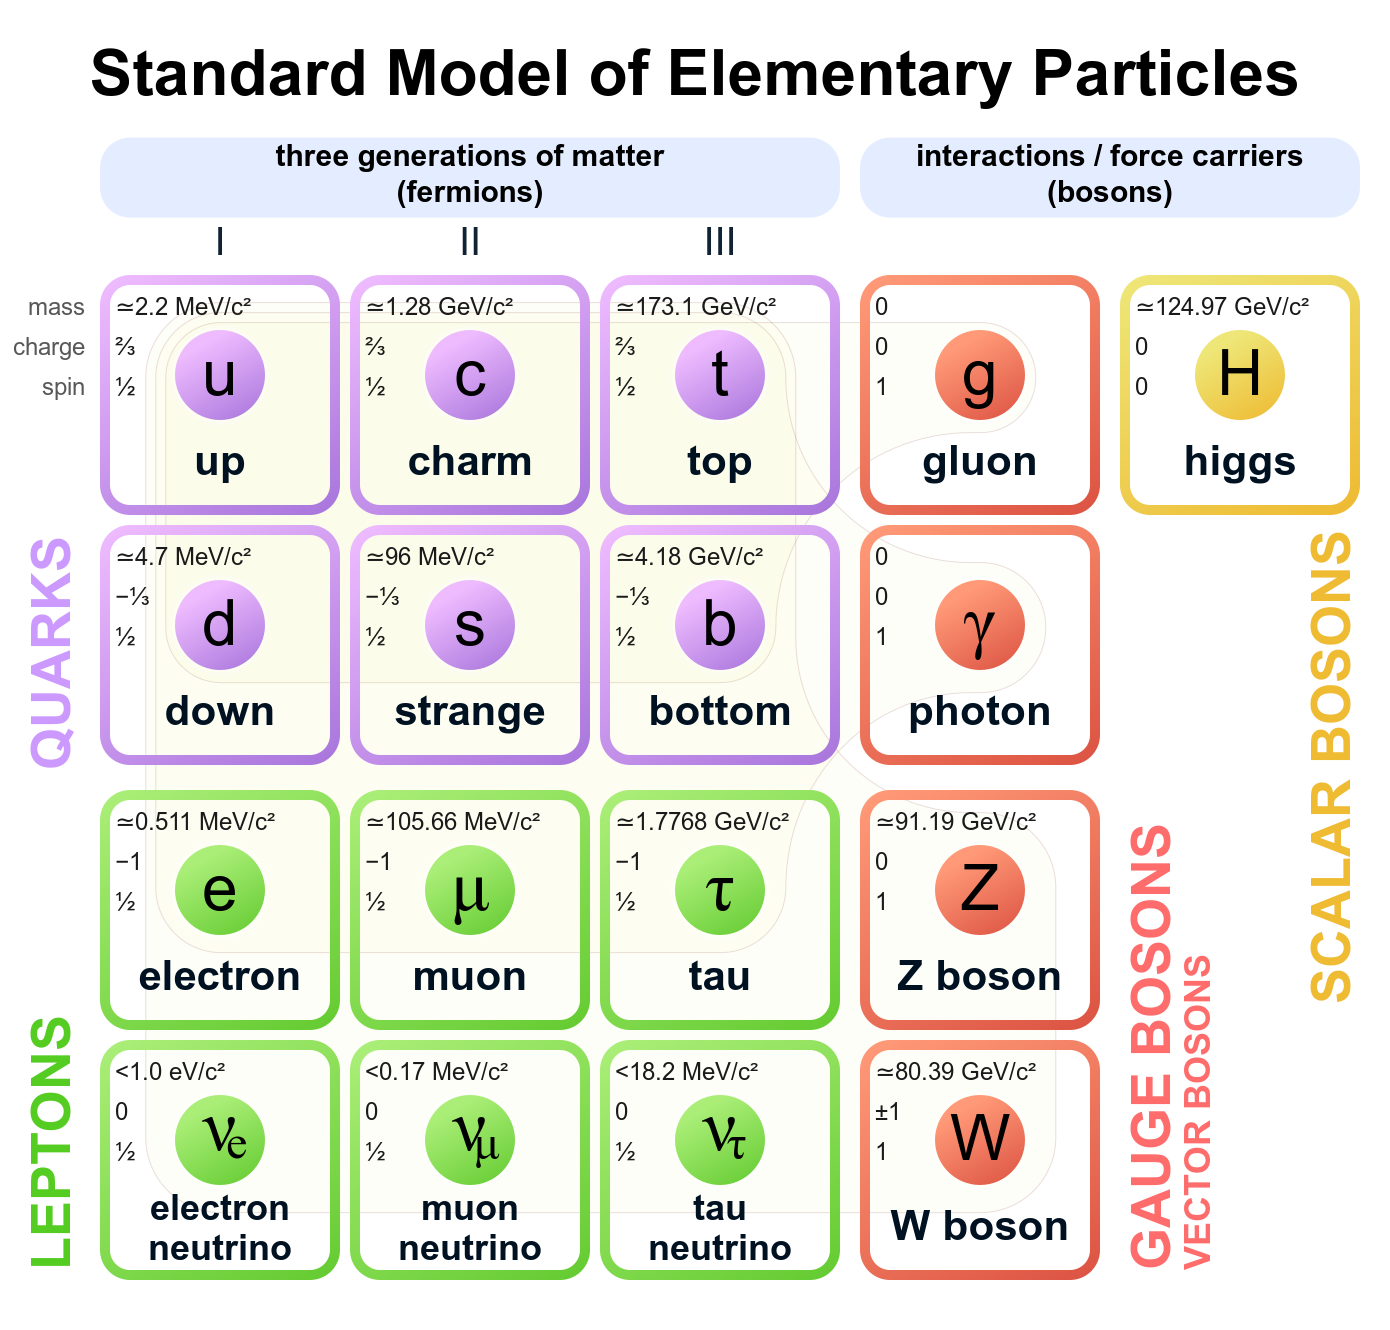
\includegraphics[width=0.5\columnwidth]{Figures/Standard_Model_of_Elementary_Particles.png}
	\caption{Particle content of the Standard Model of Particle Physics. For each particle, the mass, the charge and the spin are reported. Please bear in mind that the mass of light quarks ($u$, $d$, $s$) is not straightforward to define and estimate, given that no free quark can be observed. Taken from Ref.~\cite{SM_wikipedia}.}
		\label{tab:SM}	
\end{figure}


\section{The Standard Model of Particle Physics} 

The best theory of particle physics we have available is the so--called Standard Model of Particle Physics (SM in the following). It specifies the full list of particles, their properties and their interactions. Table~\ref{tab:SM} summarises the particle content of the SM. There are three leptonic families (in green). In each leptonic family, there is a charged lepton and a neutrino of the same flavour. There are also three quark families (in purple). In each quark family there is a quark with charge $+\frac{2}{3}$ and one with charge $-\frac{1}{3}$. Each quark defines its own flavour. Not shown in the table: for each particle family there is an identical family composed by anti-particles. So, for the family composed by the electron and its neutrino, there is a family composed by a positively charged electron (the positron) and an antineutrino, and same for the quarks. 

There are also bosons, that mediate the interactions between the particles in the leptonic and quark families (in red). These are: 
\begin{itemize}
\item The photon, that mediates the electromagnetic interaction between charged particles. 
\item The $W^+, W^{-}$ and $Z$ bosons, which mediate the weak interaction between leptons and between quarks. 
\item The gluons, that mediate the strong nuclear interaction between quarks. 
\end{itemize} 

Finally, the Higgs boson is shown in yellow: it interacts with all particles with an intensity that is proportional to the particle mass. 

We will use a helpful graphical tool to represent interactions between particles. These are the Feynman diagrams. Please bear in mind that we will use them only as a graphical tool, but they are actually a representation of quantitative mathematical expressions that allow to precisely calculate how likely a given process is to occur. In these graphs, we will always represent incoming particles on the left and outgoing particles on the right. 

There are important rules that have to be respected when drawing possible Feynman diagrams:
\begin{enumerate}
\item Electric charge, momentum, energy and angular momentum are always conserved at a vertex.
\item Fermions are represented with arrows. An incoming (in a vertex) fermion is represented with an incoming arrow, while an outgoing fermion is represented with an outgoing arrow. For anti-fermions, rules are reversed: an incoming anti-fermion is represented with an outgoing arrow, while an outgoing anti-fermion is represented with an incoming arrow. See examples in Figure~\ref{fig:feyn_example}. 
\item The total number of leptons has to be conserved. Each lepton contributes to the number of leptons with an additive $+1$, while each anti-lepton with an additive $-1$.
\item Likewise, the total number of quarks has to be conserved. Each quark contributes with an additive $+\frac{1}{3}$, while each anti-quark with an additive $-\frac{1}{3}$.
\item As a consequence of rule 1 for angular momentum, a three-line vertex can only be: two fermions and a boson; three bosons.
\item Gluons interact only with quarks and other gluons. 
\item The $Z$ and $\gamma$ bosons always conserve the flavour. So, $Ze^+e^-$, $Zu\bar{u}$, $\gamma c\bar{c}$ are perfectly legal vertices, $Z e^+ \mu^{-}$, $Zc\bar{s}$ and $\gamma e^-\mu^+$ are not.
\item The $Z$ boson does not interact with the photon.
\item The $W$ boson interaction conserves the leptonic flavour. So $We\bar{\nu}_e$ is a legal vertex, but $We\bar{\nu}_{\mu}$ is not. 
\end{enumerate}

Figure~\ref{fig:feyn_example}~\footnote{In this handbook, we will always deal with so-called \textit{leading-order} Feynman diagrams. If you want to know more about \textit{higher order} Feynman diagrams, please consult Ref.~\cite{shaw}. We will also neglect possible leading order Feynman diagram vertices that include more than three lines.} shows examples of allowed Feynman diagrams, while Figure~\ref{fig:forbidden_feyn} shows some processes which are not allowed. 

 \begin{figure}[!h]
\begin{center}
\subfigure[Production of a Z boson decaying into a $\mu\bar{\mu}$ pair at an electron-positron collider.]{
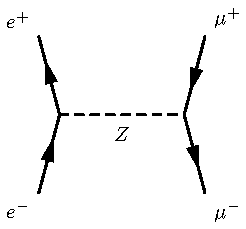
\includegraphics[width=0.2\textwidth]{./Figures/ee_to_Zmumu.eps}
}
\hfill
\subfigure[A diagram for $W$ production at a hadron collider, followed by the $W$ decay into two quarks.]{
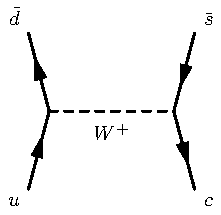
\includegraphics[width=0.2\textwidth]{./Figures/ud_to_Wcs.eps}
}
\hfill
\subfigure[A diagram for $t\bar{t}$ production at a hadron collider.]{
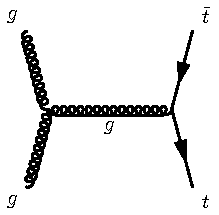
\includegraphics[width=0.2\textwidth]{./Figures/gg_to_ttbar.eps}
}
\hfill
\subfigure[Higgs boson production via the so-called gluon fusion process, followed by $H\rightarrow\gamma\gamma$, at a hadron collider. Both the gluons and the photons are massless particles, the Higgs boson couples to them through intermediate particles.]{
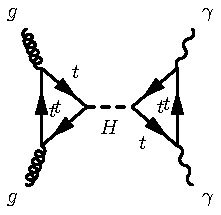
\includegraphics[width=0.2\textwidth]{./Figures/Higgs_gluonFusion.eps}
}
\end{center}
\caption{Examples of valid Feynman diagrams. For each of them, the fermion lines do not stop within the diagram, rather they enter and exit the diagram fully. This is a consequence of angular momentum and charge conservation.}
\label{fig:feyn_example}
\end{figure}

 \begin{figure}[!h]
\begin{center}
\subfigure[Violation of charge conservation at the $W$ production vertex.]{
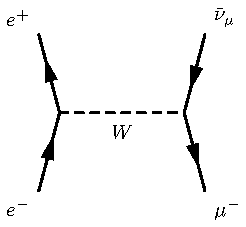
\includegraphics[width=0.2\textwidth]{./Figures/ee_to_Wmumu.eps}
}
\hfill
\subfigure[Flavour violation at the $Z$ decay vertex. The $Z$ boson only couples to leptons and quarks of the same flavour.]{
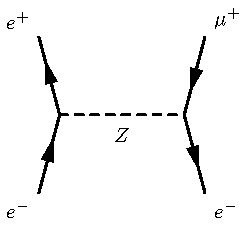
\includegraphics[width=0.2\textwidth]{./Figures/ee_to_Zemu.eps}
}
\hfill
\subfigure[Charge conservation violation at the Higgs boson production vertex.]{
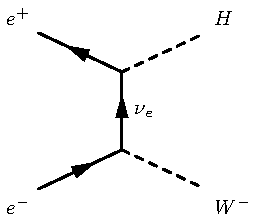
\includegraphics[width=0.2\textwidth]{./Figures/ee_to_WH.eps}
}
\hfill
\subfigure[Four-fermion interaction vertices do not exist in the Standard Model.]{
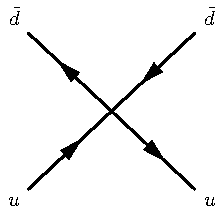
\includegraphics[width=0.2\textwidth]{./Figures/ud_to_ud.eps}
}
\hfill
\subfigure[There is a broken fermion line at both vertices (violation of charge, angular momentum, baryon number conservation).]{
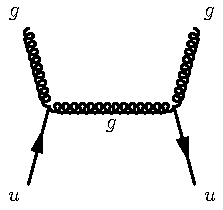
\includegraphics[width=0.2\textwidth]{./Figures/ug_to_g.eps}
}
\hspace{1cm}
\subfigure[The Higgs boson does not couple directly with particles with no mass.]{
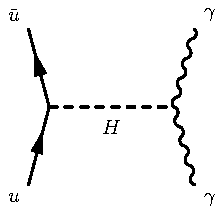
\includegraphics[width=0.2\textwidth]{./Figures/uu_to_Hgamgam.eps}
}
\end{center}
\caption{Examples of processes which are {\color{red} NOT} allowed in the Standard Model, with a quick explanation of why they are not allowed.}
\label{fig:forbidden_feyn}
\end{figure}



\section{Special relativity and units}

In particle physics it is customary to choose a system of units in which the value of the Planck constant $\hbar$ and the speed of light $c$ are both set to unity: $\hbar = c = 1$. Energy and momentum are therefore measured with the same units. Often the electronvolt (eV) is the energy unit chosen. For the applications of this experiment, we will be using MeV, GeV and TeV. Because of the Heisenberg uncertainty principle, the unit for space is also fixed: 

\begin{align}
\Delta p \Delta x \sim \hbar = 1 \implies [x] = \frac{1}{[p]}  = \frac{1}{\mathrm{MeV}}
\end{align}

Likewise, from $\Delta E \Delta t \sim \hbar = 1$, it follows that time has the same units of space. From $E=mc^2$, it follows that mass and energy have the same units. 


The particle free motion is described in terms of their energy $E$ and momentum $\mathbf{p}$. The three momentum components and the energy form a so-called 4-vector. You already have the knowledge of what a 4-vector is, but probably nobody has used this name just yet. Let's start from a standard position vector in space $\mathbf{x}$, with components $(x,y,z)$ in a given reference frame $S$. Let's name this a 3-vector (and you can probably already guess where I am going...). You know well that in special relatively the spacial coordinates and the time of a given event cannot be treated independently from each other, simply because they mix if one describes the same event from a different reference frame in uniform motion with respect to the original one.  For a change of reference frame from a frame $S$ to one $S'$ moving with speed $v$ along $\hat{x}$ with respect to $S$, the 4-vector transforms into $(\mathbf{x'},t')$ such that:

\begin{align}
x' &= \gamma \left(x + \beta t\right) \nonumber \\
y' &= y \nonumber \\
z' &= z \nonumber\\
t' &= \gamma \left(t + \beta x\right)
\end{align}
\label{eq:lorentz_transform}

\noindent where we are using units in which the speed of light $c$ is equal to 1. $x'$ is a function of both $x$ and $t$, and the same is true for $t'$.  Perfect! Let's then define a 4-vector as $x_\mu = (x,y,z,t)$. The components of a 4-vector transform by Lorentz boost as in Eq.~\ref{eq:lorentz_transform}.

The symbols $\gamma$ and $\beta$ are defined (for $c=1$) by: 

\begin{align}
\gamma = \frac{1}{\sqrt{1-v^2}} \qquad \beta = \frac{v}{c} = v
\end{align}

The transformations in Eq.~\ref{eq:lorentz_transform} are such that the product  

\begin{align}
s = t^2 - \mathbf{x} \cdot \mathbf{x}
\end{align}

\noindent is invariant for Lorentz transformations, that is, its value is the same in the reference frame $S$ or in any other boosted frame $S'$. 

\begin{exercise}
Prove it! Prove that  $t^2 - \mathbf{x} \cdot \mathbf{x} =  t'^2 - \mathbf{x'} \cdot \mathbf{x'}$, where the primed quantities are connected to the non-primed ones by a Lorentz transformation like in eq.~\ref{eq:lorentz_transform}
\end{exercise}

So, momentum and energy form another 4-vector, $p_{\mu} = (p_x,p_y,p_z,E)$. That means that if I go from one reference frame to another in relative motion along $\hat{x}$,

\begin{align}
p_x' &= \gamma \left(p_x + \beta E\right) \nonumber \\
p_y' &= p_y \nonumber \\
p_z' &= p_z \nonumber\\
E' &= \gamma \left(E + \beta p_x\right)
\end{align}
\label{eq:lorentz_transform_momentum}

It also means that $E^2 - \mathbf{p}\cdot \mathbf{p}$ is an invariant.......

\subsection{Invariant Mass}
\label{sec:invariant_mass}

The fact that for a 4-vector of type $\left(\mathbf{m}_x, m_t\right)$ the product $s_{m} = m_t^2 - \mathbf{m}_x \cdot \mathbf{m}_x$ is Lorentz-invariant (that is, it is the same in every reference frame, regardless of its boost) is general. The number $\sqrt{s_{m}} = \sqrt{m_t^2 - \mathbf{m}_x \cdot \mathbf{m}_x}$ is the \textit{magnitude} of the 4-vector. As pointed out earlier, the energy and momentum form a 4-vector $\left(\mathbf{p},E\right)$. Therefore the combination $s = E^2-p^2$ (where $p$ indicates the magnitude of $\mathbf{p}$) is Lorentz-invariant. What is the value of this Lorentz-invariant quantity? Let's consider a particle of mass $m$. In its own rest frame: 

\begin{align} 
E &= m \\ 
\mathbf{p} &= 0 \\ 
s^2 &= E^2 - p^2 = m^2
\end{align}

\noindent But since $s^2$ is Lorentz-invariant, \textit{this mathematical combination of the momentum and the energy of the particle will yield the particle mass regardless of the rest frame where it is computed!}. We will use this fact repeatedly.

\section{Proton-proton Collisions - Collider Physics Variables}
\label{sec:collider_physics_variables}

In this experience, we will study proton-proton collisions produced by the LHC and recorded by ATLAS. The LHC collides two beams of protons head-on. The energy of the protons in each beam is $\ebeam = 6.5\ \TeV$. 

As said earlier, protons are not elementary particles. They are made by three \textit{valence} quarks (two $u$ and one $d$) and a \textit{sea} of other quark-antiquark pairs and gluons, which are created and destroyed continuously according to quantum mechanics. All these particles (the valence quarks and the sea quarks and gluons) take the generic name of \textit{partons}. 

The scale for the proton binding energy is given by its own mass ($\sim 1\ \GeV$). With respect to the typical energy transfer in a LHC collision of interest, with energy exchanged of hundreds of GeV, the binding energy of the proton is small. Therefore the partons in the proton in a LHC collision \textbf{can be considered as free}: the LHC is indeed a parton collider. 

Partons inside a proton however do not have the same energy/momentum as the proton of course: it is the sum of the energies and momenta of all partons that will yield the energy and momentum of the proton. Let's say that each parton $i$ in the collision carries a fraction $x_i$ of the momentum and energy of the proton. The 4-vectors of the protons and colliding partons are (neglecting all masses, and setting the $\hat{z}$ as beam axis) 

\begin{align}
\mathrm{Proton 1}&: \left(0,0,\ebeam,\ebeam\right) \\
\mathrm{Proton 2}&: \left(0,0,-\ebeam,\ebeam\right) \\
\mathrm{Parton 1}&: \left(0,0,x_1\ebeam,x_1\ebeam\right) \\
\mathrm{Parton 2}&: \left(0,0,-x_2\ebeam,x_2\ebeam\right) \\
\end{align}

The magnitude of the 4-vector corresponding to the sum of the two proton 4-vectors is 

\begin{align}
\sqrt{s} = \sqrt{\left(2\ebeam\right)^2 - \left(\ebeam-\ebeam\right)^2} = \sqrt{4\ebeam^2} = 2\ebeam = 13\ \TeV
\end{align}

\noindent which is known as the centre-of-mass energy of the LHC. However, this is \textbf{not} the centre of mass energy of the parton-parton collisions! The actual particles colliding are the partons. Their own centre-of mass energy is:

\begin{align*}
\sqrt{\hat{s}} = \sqrt{\left( x_1 + x_2 \right) ^2 \ebeam^2 - \left( x_1 - x_2\right)^2 \ebeam^2}
\end{align*}

\begin{exercise}
Prove that this implies $\sqrt{\hat{s}} = \sqrt{x_1 x_2} \sqrt{s}$
\end{exercise}

By the way: the frame in which the proton-proton collision happens at rest (the laboratory frame) does not coincide with that in which the parton collision happens at rest. With respect to the laboratory frame, the parton-parton collision happens in a system which is boosted along the beam axis by $p_{\mathrm{boost}} = |x_1-x_2| \ebeam$.

 \begin{figure}[!h]
\begin{center}
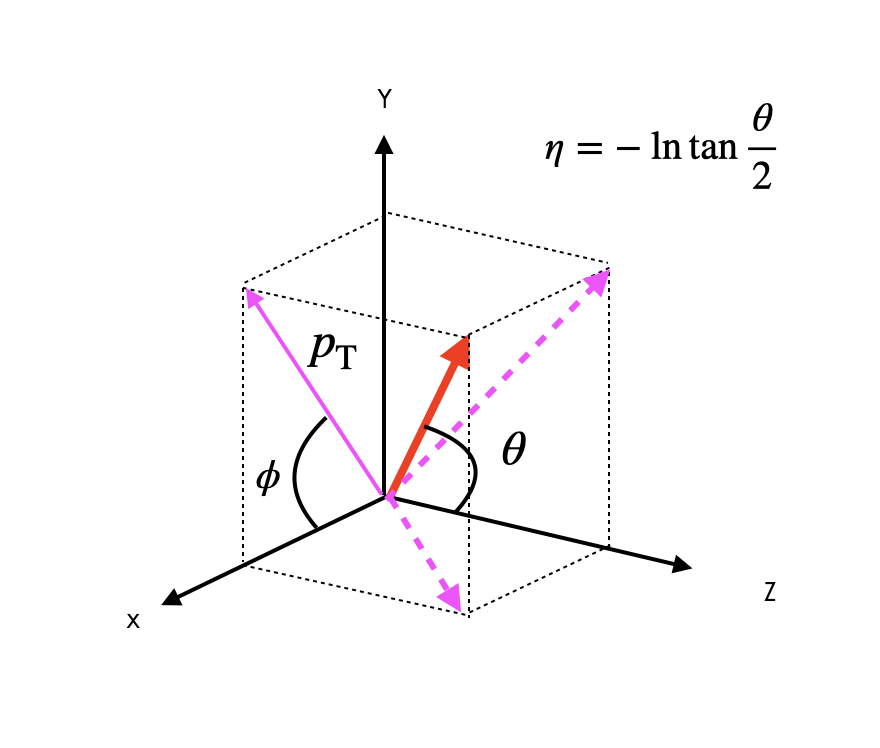
\includegraphics[width=0.5\textwidth]{./Figures/collider_physics_variables.png}
\end{center}
\caption{Diagram of the kinematic variables used at a hadron collider. The $z$ axis coincides with the beam axis.}
\label{fig:collider_variables}
\end{figure}


Let's recap: on an \textbf{event-by-event basis}, the parton-parton collision happens in a frame with a different boost with respect to the laboratory frame, and the collision energy is smaller than the nominal proton-proton centre-of-mass energy. 

\begin{exercise}
The mass of the top quark is 172 GeV. The SppS, a collider colliding protons and antiprotons at CERN, worked up to energies of $\sqrt{s} = 900\ \GeV$. Yet, we had to wait for the Tevatron ($\sqrt{s} = 1.8\ \TeV$) for the top quark discovery. Why?
\end{exercise}

\begin{exercise}
Draw one of the most relevant Feynman diagram for the production of the following particles at the LHC. If quarks are involved, specify if they are likely to be valence or sea quarks: $Z$ boson production, $W$ boson production, $t\bar{t}$ production.
\end{exercise}

\begin{exercise}
The mass of the $W$ boson is $m = 80\ \GeV$. In a given collision pp collision at $\sqrt{s} = 13\ \TeV$, the $W$ boson is produced by a collision of a valence quark with $x = 0.3$,  and a sea quark. Find $x$ of the sea quark and compute $p_{\mathrm{boost}}$ for this collision.
\end{exercise}


So, in practice what happens is that in each event, the LHC experiments look at a collision happening with an unknown boost along the $\hat{z}$ axis. There is one important implication: if we measure any variable which is not Lorentz-invariant, we would make a big confusion when measuring it in many events, because we would mix up values belonging to different reference frames! This implies we have to carefully choose the quantities that we measure at a hadron collider like the LHC to characterise the particles' final states: we should avoid using any variable relying on \textit{longitudinal} quantities, that is, quantities relying on variables measured along the $\hat{z}$ axis. The reason  Therefore, the variables we use at a hadron collider are (see also Figure~\ref{fig:collider_variables}) 

\begin{itemize}
\item The momentum in a plane transverse to the beam, $\pt$.
\item The angle $\phi$ in the transverse plane with respect to the direction pointing towards the LHC centre.
\item The mass.
\end{itemize}

And now we have a problem, because three variables do not determine a 4-vector, of course. We need somewhat to provide the direction with respect to the beam axis. This is done with the rapidity $y$ variable, or with its approximated variable (valid for massless particles) the pseudorapidity $\eta$. 

\begin{align*}
y &= \frac{1}{2} \ln \left(\frac{\mathbf{E} + p_z}{\mathbf{E} + p_z} \right) \\
\eta &= -\ln \tan \frac{\theta}{2}
\end{align*}

\section{Cross-section and luminosity}
\label{sec:cross_section_lumi}

Imagine you have a beam of particles impinging on a slab of targets, and that the targets are small enough that you can neglect shielding effects of one target with respect to another. The total number of interactions that you will observe per unit time will be determined by:

\begin{itemize}
\item characteristics of the beam of particles (how many particles per unit surface per unit time you are shooting, that is, the incoming flux of particles),
\item the target density,
\item the transverse area that the targets offer to the beam, that is, the cross-section of the individual targets. 
\end{itemize}

Inheriting this language, we define the cross-section and the luminosity of a given process at a hadron collider such that the number of occurrences of that process that we observe per unit time is given by: 

\begin{align}
\frac{dN}{dt} = \sigma \times \mathcal{L}
\end{align} 

In the example above, the luminosity is something connected with how many protons per beam we have, how many beams are circling the LHC, etc., while the cross-section is intrinsically connected with the physical interaction yielding a given process. The cross-section units are those of a surface (cm$^2$, for example\footnote{Particle physics cross sections are normally expressed in barns, where $1\ \mathrm{barn} = 10^{-24}\ \mathrm{cm}^2$}), while those of the luminosity are

\begin{align}
[\mathcal{L}] =  [\mathrm{surface}]^{-1}\cdot [\mathrm{time}]^{-1}.
\end{align}

A typical number $\mathcal{L}$ during the LHC Run 2 is $\mathcal{L} \sim 2\times 10^{34}$ cm$^{-2}$ s$^{-1}$. The total number of events we will count for a given process in a given period of time is of course given by 

\begin{align}
N = \int_{\Delta T} \frac{dN}{dt} dt = \int_{\Delta T} \sigma \times \mathcal{L} dt &= \sigma \int_{\Delta T} \mathcal{L} dt = \sigma \Lint, \\ 
\Lint &= \int_{\Delta T} \mathcal{L} dt.
\end{align}

The data collected by a given experiment over a period of time are typically expressed with the corresponding \textit{integrated luminosity} $\Lint$. Let's make an example. The ATLAS experiment has collected a number of proton-proton collisions corresponding to $\Lint = 139\ \ifb$ during the so-called Run 2 at $\sqrt{s} = 13\ \TeV$. The production cross-section for top pairs is predicted to be $\sigma_{t\bar{t}} = 831\ \mathrm{pb}$. Let's compute how many top pair production events we expect to have collected during the full Run 2: 

\begin{align}
N_{t\bar{t}} = \sigma_{t\bar{t}} \times \Lint &= 831 \times 10^{-12} \ \mathrm{barns} \times 139 \times \left(10^{-15}\ \mathrm{barns}\right)^{-1} \\
N_{t\bar{t}} &= 1.16\times 10^{8}
\end{align}

So, we expect something like 116 million top pairs to have been produced during Run 2 in ATLAS. 

\begin{figure}[tb] 
	\begin{center}
	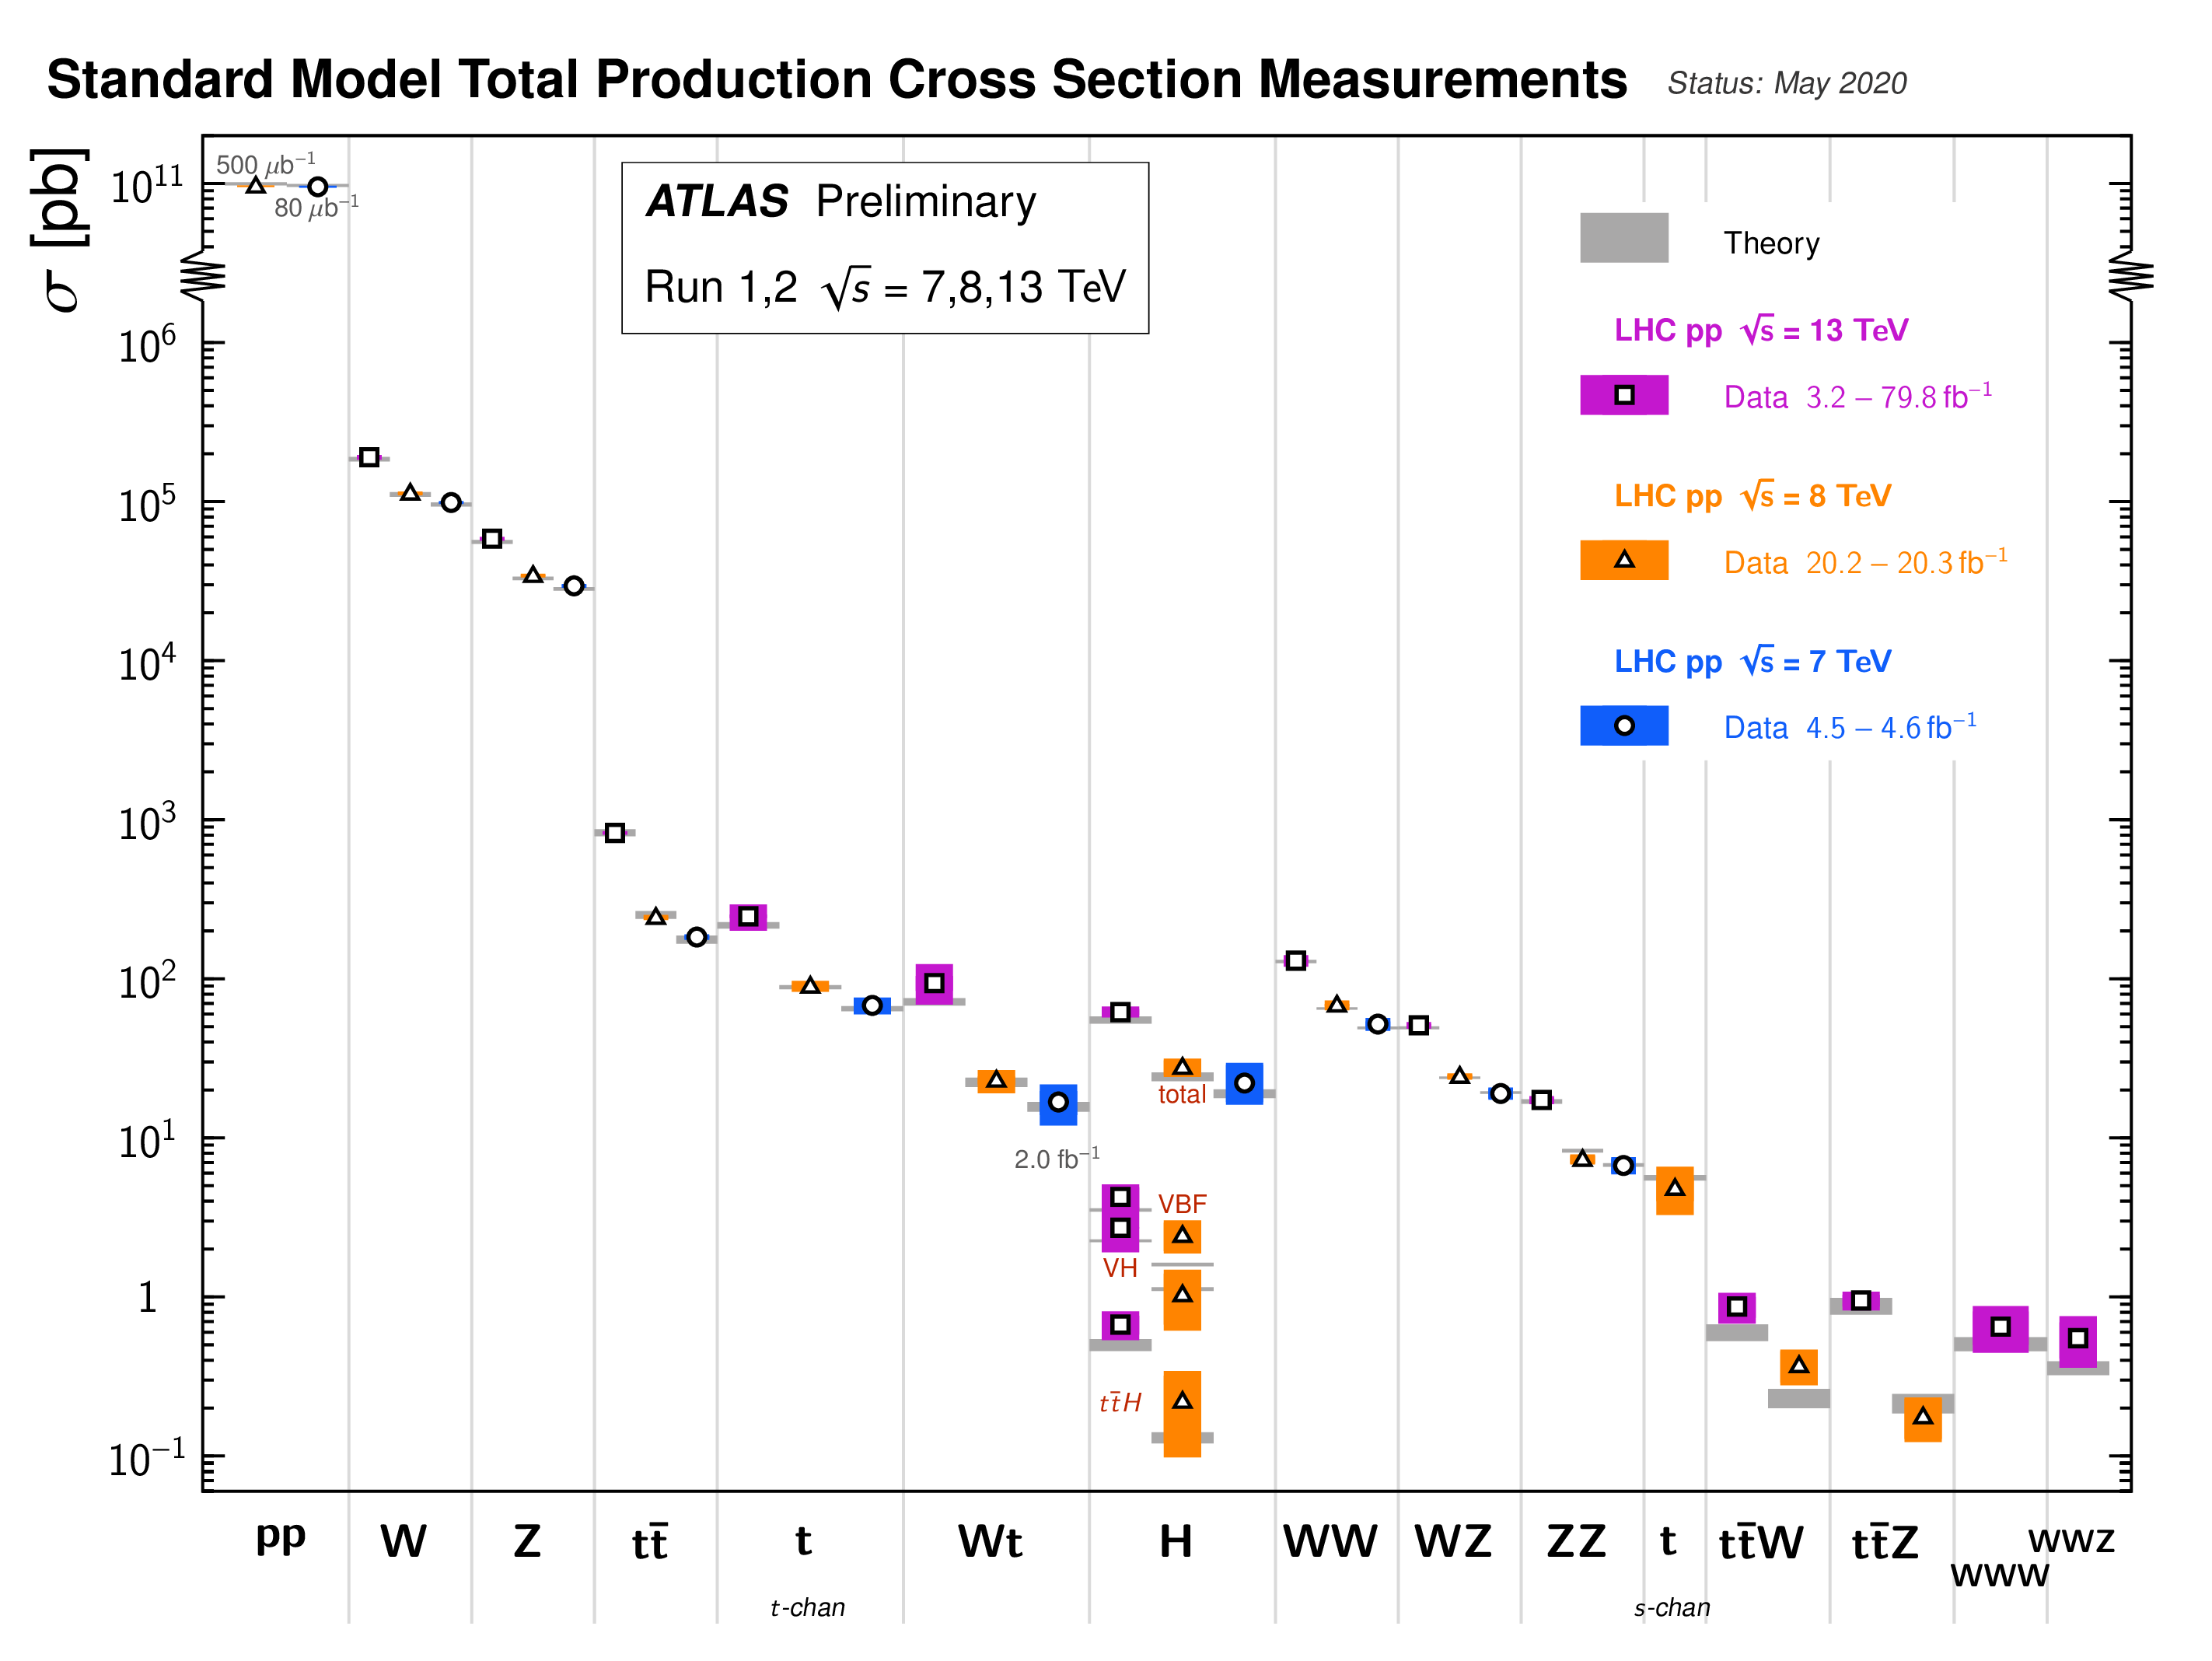
\includegraphics[width=0.7\columnwidth]{Figures/SM_summary.png}
	\end{center}
	\caption{Predictions and ATLAS measurements for the production cross sections of several Standard Model processes. Taken from Ref.~\cite{SM_summary}.}
	\label{fig:SM_summary_plot}
\end{figure}

Now, let's take a close look at Figure~\ref{fig:SM_summary_plot}. It shows the cross-sections for several SM processes at the LHC, for different proton-proton centre-of-mass energies. The proton-proton inelastic cross-section at $\sqrt{s} = 13\ \TeV$ is about $80$ mb. Let's consider one random process as an example, say $WW$ production. The plot tells us that the production cross section is between 100 and 200 pb - let's take 160 pb. So, from the ratio of these numbers, we learn that only one in 500,000 proton-proton collisions will produce $WW$. 

\begin{exercise}
From Figure~\ref{fig:SM_summary_plot}, the Higgs boson production cross-section is $\sigma = 80$ pb. Compute how many Higgs bosons LHC has produced during Run 2, and using the typical value for $\mathcal{L}$ given above, compute how many Higgs bosons per minute the LHC is producing when running at that luminosity. 
\end{exercise}


\chapter{ATLAS}
\label{sec:ATLAS}
% !TEX root = ../main_orange.tex

We will now go though the main aspects of how different particles are reconstructed by ATLAS. This discussion will be crucial to understand the variables that are available for this experiment. 

\section{The ATLAS detector}

ATLAS is a general-purpose particle detector operating at a hadron collider. The structure of the detector is sometimes referred to as onion-like, because different layers of detectors are present when going from the collision point outwards. A detailed description of the ATLAS detector and the technologies used for particle detection goes well below the scope of this document: if you are interested please refer to Ref.~\cite{Aad:2008zzm}. What we will do here is to summarise the main principles behind particle detection.

\begin{figure}[tb] 
	\centering
	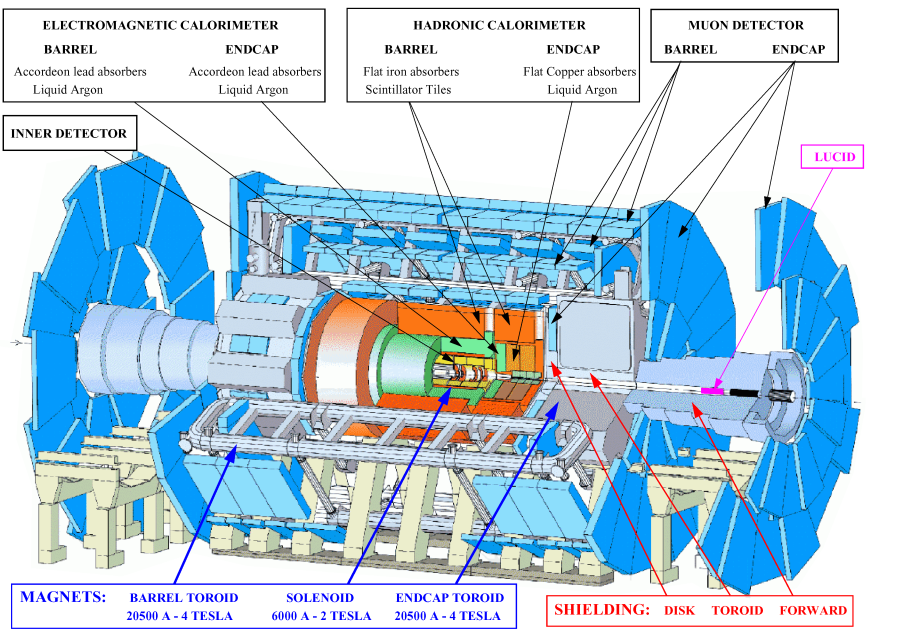
\includegraphics[width=0.7\columnwidth]{Figures/atlas.png}
	\label{fig:ATLAS}
	\caption{Overview of the ATLAS detector. Taken from Ref.~\cite{ATLAS_detector_image}}
\end{figure}

Figure~\ref{fig:ATLAS} shows the various components of ATLAS. Starting from the collision point and going outward: 

\begin{itemize}

\item \textbf{Inner Detector (ID):} Starting at about 3 cm away from the collision point, the inner detector is optimised to measure the position of charged particles. It is immersed in a magnetic field directed along the $z$ axis, such that charged particles trajectories are bent. From the curvature radius it is possible to measure the particle momentum transverse to the magnetic field. 

\begin{exercise}
Remembering that $\mathbf{F} = q \mathbf{v} \times \mathbf{B}$ is acting as centripetal force, estimate the curvature radius of a particle with unit charge and momentum $p = 10\ \GeV$ if $B = 2$~T. 
\end{exercise}

\item \textbf{Electromagnetic (EM) calorimeter:} It stops electrons and photons and measures their energy. It also participate in the energy measurement of hadrons. 
\item \textbf{Hadronic (HAD) calorimeter:} Together with the electromagnetic calorimeter, it measures the energy of neutral and charged hadrons. 
\item \textbf{Muon spectrometer (MS):} Muons and neutrinos are the only particles in the SM that are able to exit the ATLAS calorimeters. The principle of the muon spectrometer is similar to that of the inner detector: the position of muons is measured several times while they are bending in a magnetic field generated by the air-core toroids. From that, a second measurement of the muon momentum is performed, which is typically  combined with the first one taken by the ID. 
\end{itemize}

The subdetectors outlined above are used in combination to reconstruct a number of different final state ``objects''. The number of types of objects which is normally used in an analysis is actually relatively limited. The main features of each of these objects is reviewed below. 

\begin{itemize}
\item{Electrons:} they are identified by a cluster of energy in the EM calorimeter matched with a track in the ID. \textit{Shower shape variables} (that is, the shape of the cluster in the calorimeter), the track quality, and the quality of the matching between the cluster and the track (are the track momentum and cluster energy compatible?) determine the identification. 
\item{Photons:} similar to electrons for the cluster in the EM calorimeter, but with no associated track in the ID. 
\item{Muons:} a track in the MS is almost uniquely identifying a muon (no other charged particle pass through the calorimeters). Typically the MS track is matched to one in the ID. 
\item{Jets:} Quarks and gluons cannot emerge from a collision as such. They go through a process of fragmentation and hadronisation~\cite{fragment_hadronise}, resulting in a jet of collimated hadrons, whose total momentum and direction resembles that of the originating quark/gluon. Such jets are reconstructed mainly from the HAD and EM calorimeter information, but they use some information from the ID as well. 
\item{$b$-jets:} $b$-quarks have a longer lifetime than the other quarks. They travel of the order of a cm or less before decaying. The presence of such secondary vertex (that is, a vertex that does not coincide with the primary one from the pp collision in the transverse plane) can be exploited to ``tag'' the jet as originating from a $b$.
\item{$\tau$ leptons:} The lifetime of the $\tau$ is extremely short. For all practical purposes, it decays before producing any visible effect in the detector. There are two main categories of $\tau$ decays: the leptonic ones and the hadronic ones. If a $\tau$ decays to an electron and muon (through $\tau\rightarrow \ell \bar{nu}_{\ell} \nu_{\tau}$ to conserve the lepton number and flavour), it will be seen as a lepton in the detector. If instead a tau decays to hadrons, then it looks like a very narrow jet with few tracks attached, and it can be identified based on these characteristics. 
\item{Invisible particles:} If an invisible particle is produced (neutrinos, in the standard model), their presence is inferred from the measurement of the total momentum transverse to the beam. Given that the momentum in the plane transverse to the beam is zero before the proton-proton collision, it has to be zero after the collision. The negative vectorial sum of the transverse momenta of all object in the events is called the \textit{missing transverse momentum}, and is an estimate of the total transverse momentum of invisible particles.   
\end{itemize}

Figure~\ref{fig:ttbar_eventdisplay} shows a candidate event for $t\bar{t} \rightarrow \mu \nu_{\mu} + 4\ \mathrm{jets}$. See the caption for further details. 

\begin{figure}[tb] 
	\centering
	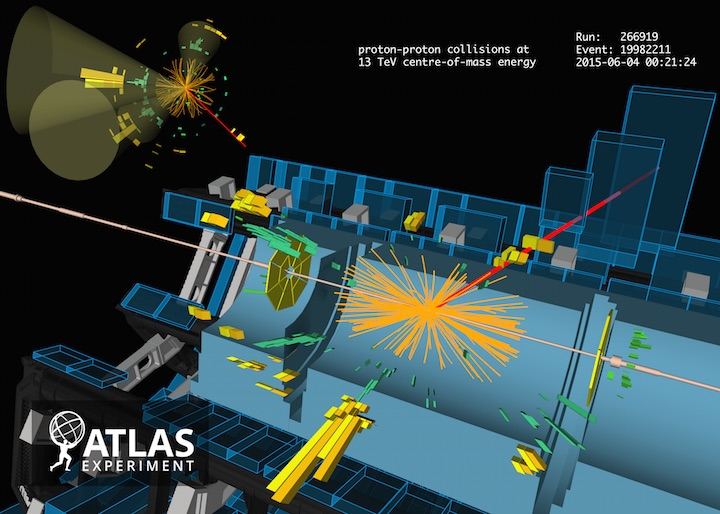
\includegraphics[width=0.7\columnwidth]{Figures/ATLAS_ttbar_candidate_13TeV_VP1_run266919_evt19982211_thumb.jpg}
	\label{fig:ttbar_eventdisplay}
	\caption{Display of a $t\bar{t}$ candidate event from proton-proton collisions recorded by ATLAS at a collision energy of 13 TeV. The red line shows the path of a muon with transverse momentum around 35 GeV through the detector. The green and yellow bars indicate energy deposits in the EM and HAD. From close-by deposits in these calorimeters, four jets are identified with transverse momenta between 25 and 80 GeV. Taken from Ref.~\cite{ATLAS_ttbar_evtdisplay}}
\end{figure}

\section{Monte Carlo and real events}

In this experiment you will deal with two types of events: simulated and real ones. The simulated ones are often referred to as Monte Carlo, or simply MC, events. MC events are the result of a computer simulation, that emulates at best the theory we have for the proton-proton collision. They simulate a specific process (like $Z$ production, or $H$ production), they save the so called truth-level information (that is, the particles that were produced in the collision and that enter the detector) and they also simulate the response of the detector (reco-level). The MC represents our theoretical prediction. 

%It is probably worth at this stage to introduce the concept of cross-section weight. Suppose that I simulate $N$ events of a process whose cross-section is $\sigma$. I know that the data I will be looking at correspond to an integrated luminosity $L$. If I want 



\chapter{Open data: practical guide}
\label{sec:open_data}
% !TEX root = ../main.tex

The ATLAS open data consist in a set of MC and real events that the ATLAS collaboration has released for open use. The main web page where they are introduced is \url{http://atlas.cern/resources/opendata}. Please spend some time on this page, explore it, play with it.

The next step is to actually do something. In the ``Online Open Data Analysis'' section of the page, click on ``Analyse ATLAS Open Data with Jupyter Notebooks'', and then in the jupyter-looking window select ``13-TeV-examples'', then "uproot\_python". You should get to this \href{https://notebooks.gesis.org/binder/jupyter/user/atlas-outreach--ection-opendata-hbw4boy5/notebooks/13-TeV-examples/uproot_python}{page}. 

Each notebook corresponds to a different analysis. Please open \verb|HZZAnalysis.ipynb|.

\chapter{Experiments}
\label{sec:experiments}
% !TEX root = ../main.tex



\subsection{Experiment 1: Understanding $H\rightarrow 4\ell$}

In this experiment we will dig deeper into the $H\rightarrow ZZ$ analysis that we have seen earlier. Please document everything you do, including the answers to the questions below, in your logbook. It is suggested you make a copy of the HZZAnalysis.py before you start to modify it.

\begin{enumerate} 
\item Edit the file to print the histogram integrals of the different processes: $ZZ\rightarrow 4\ell$ (red histogram), $Z$ and $\ttbar$ production (shown together in purple), $H\rightarrow ZZ$ (cyan), and, finally, the data. From the discussion about MC weights in Section~\ref{sec:review_notebook}, it should be clear that the integral of the histograms and the actual number of events are different for MC (because of all the applied weights), while they will coincide for the data. 
\item Validate these printouts: try to have a rough estimate of those integrals by looking at the output histogram of the code. Make sure that the rough estimate and the exact printouts are in the same ballpark.
\item Compute the total expected background $B$ by summing the integrals of the $ZZ$, $Z$ and $\ttbar$ processes. We will now compute its agreement with the observed data yield $O$: 
\end{enumerate}

\begin{mybox}
\begin{itemize} 
\item The total background $B$ represents the number of events that one \textit{expects}. Suppose I expect 100 events: the outcome of the actual experiment in general will not be exactly 100. \textit{Assuming that the background expectation is correct}, the probability of a given outcome will be described by a Poisson probability function. 
\item Please review the properties of a Poisson probability function. What is the RMS of a Poisson distribution of mean value $\mu$?
\item Evaluate the level of compatibility of your data yield $O$ by computing the probability $p(O \ge B)$ (if $O<B$, define $p = 0.5$). Such probability is known as a $p$-value. What is the p-value? Small values of the $p$-value indicate low level of compatibility of the hypothesis tested (in this case that the observed yield comes from an expected background level $B$). 
\item Physicists like to convert $p$-values. This conversion can be done for example using \href{https://planetcalc.com/7803/}{this web site}. A high $z$ score, or significance, corresponds to a low level  compatibility of the hypothesis tested (in this case that the observed yield comes from an expected background level $B$). What is the significance in this case?
\end{itemize}
\end{mybox}

\begin{enumerate}[resume]
\item Repeat the points above, but this time compute the background and the observation only in the invariant mass range $120\ \GeV < m_{4\ell} < 130\ \GeV$. What are the p-values and the significance now? 
\item Assume that the difference between the background and observation in the range  $120\ \GeV < m_{4\ell} < 130\ \GeV$ is now a yield due to $H \rightarrow 4\ell$. Knowing that the fraction of Higgs boson production that you select with this analysis is $\epsilon = 2 \times 10^{-5}$ (coming from $BR(H\rightarrow ZZ)=2.6\times 10^{-2}$, $BR(Z\rightarrow \ell\ell) \sim 6\%$, where $\ell = e, \mu$, plus some inefficiency in reconstructing leptons), what is your estimate for the production cross-section of the Higgs boson? Do your best to associate an error to it coming from the number of observed events, and compare to the standard model best prediction of $\sigma(H) = 55$ pb at $\sqrt{s} = 13\ \TeV$, with an uncertainty of 5\%. 
\item Assuming your estimate for the signal and background, how much integrated luminosity would you need to declare a $5\sigma$ discovery?
\end{enumerate}

\subsection{Experiment 2: Plot the di-electron and di-muon invariant mass in data}

In this experiment we will try to use data only to plot the di-lepton invariant mass in events with two leptons, and we will se what the meaning of the cuts on isolation on lines 27 and 31 of \verb|HZZCuts.py| actually do. Finally, we will try to understand the mass resolution for the measurement of $Z\rightarrow e^+e^-$ and $Z\rightarrow \mu^+\mu^-$. We will start from a copy of \verb|HZZAnalysis.py| and associated modules and heavily modify them. To start with, copy \verb|HZZAnalysis.py|, \verb|HZZCuts.py|, \verb|HZZHistograms.py|, \verb|HZZSamples.py|, into new files \verb|ZeeAnalysis.py|, \verb|ZeeCuts.py|, etc. 

\begin{mybox}
\textbf{TIP:} When modifying and playing with the code, reduce \verb|fraction| to something like 0.1 or even lower, to speed up the code while debugging.
\end{mybox}


\begin{enumerate} 
\item Edit the ntuple path to point to the 2lep events rather than the 4lep ones. 
\item Change the Histograms to show only one variable, $m_{ee}$ and plot it from 0\ \GeV to 200\ \GeV in log scale. 
\item Change the cuts file to have only one cut, where you reject events if the leading two leptons are not electrons of opposite charge. 
\item Change the samples to have only the data ones. 
\item Adapt the plotting code to plot only the data. 
\item Add a variable to the DataFrame ($m_{ee}$), similar to what was done with $m_{4\ell}$ in the \verb|HZZAnalysis.py| example.
\item Plot the $m_{ee}$. 
\end{enumerate}

\begin{mybox}
The histogram should display a peak at about 90 GeV, with a lot of events at different masses. The peak at 90 GeV is clearly due to $Z\rightarrow e^+ e^-$, but.... what are all other events?
\end{mybox}

\begin{enumerate} [resume]
\item  Try to add cuts that select on the lepton isolation variables, looking at the examples in  \verb|HZZCuts.py|. What you want is to reject events where either the first or the second leading lepton is not isolated. 
\item Plot again the invariant mass. Comment on differences that you see, especially at small values of $m_{ee}$. 
\end{enumerate}

\begin{mybox}
There are two main categories of leptons that the detector sees: genuine leptons and fake leptons. Genuine leptons are those where reconstruction correctly identifies a lepton as such. Fake leptons are those where the reconstruction thinks there is a lepton, but in fact there wasn't. 

Genuine leptons, in turn, are divided into two categories: prompt leptons arise from an on shell $W$ or $Z$ going to leptons (like in $pp\rightarrow Z\rightarrow e^+ e^-$, or $\ttbar \rightarrow WWbb \rightarrow \mu \nu_{\mu} jjbb$). These leptons are \textit{isolated}, that is, normally do not have other particles nearby. Non-prompt leptons are emitted in hadrons decay, like $B_0\rightarrow e^-\nu K^+$, and they tend to be non-isolated. Isolation is a powerful variable to reject fake and non-prompt leptons.   
\end{mybox}

\begin{enumerate} [resume]
\item Fit the $Z$ peak in data with a gaussian. Now repeat the analysis selecting muons instead of electrons, and fit the $Z\rightarrow \mu\mu$ peak with a gaussian. Compare the widths of the two gaussians. Which one is larger? Can you try to guess why?  
\end{enumerate}

\subsection{Experiment 3: Understanding the events outside the mass window}

In this experiment we will start from the previous one and understand what the other non-$Z$ events in the di-lepton sample actually are. Let's focus on the sample with two opposite charge electrons in the final state. 

\begin{mybox}
\textbf{TIP:} When modifying and playing with the code, reduce \verb|fraction| to something like 0.1 or even lower, to speed up the code while debugging.
\end{mybox}


\begin{enumerate} 
\item Change the Histograms file to add a missing et plot. The range will need to be something like 0\ \GeV to 300\ \GeV in log scale. 
\item Change the samples list to include \ttbar, and diboson ($WW$, $WZ$ and $ZZ$, with DSID in the range 363356 to 363493 - select those that contain two leptons) production.   
\item Modify the plotting code to include the MC, similarly to what you had for \verb|HZZAnalysis.py|
\item Plot the $m_{ee}$ and $E_{T}^{miss}$.
\item Add a cut to reject events with $m_{ee}$ on the $Z$ peak. Plot again the $E_{T}^{miss}$. 
\item Comment about the results. What are the events which are not $Z$ in this data sample? Why do they tend to have a larger missing transverse momentum than $Z$ events?  Plot the expected composition of the data (what fraction is $Z$, what fraction is the rest) for $ E_{T}^{miss} > X$ as a function of $X$.
\end{enumerate}

\begin{mybox}
\textbf{Bonus task:} DSIDs from 392501 to 392521 contain events from physics processes which are not foreseen by the Standard Model, but by some extension of it. Do you want to try and see whether you will be able to discover new physics using the ATLAS Data? Those new processes are $pp\rightarrow \tilde{\chi}^+_1  \tilde{\chi}^-_1 \rightarrow 2\tilde{\chi}^0_1 2\nu \ell^+\ell'^-$. All you need to know is that the new particle $\tilde{\chi}^0_1$ behaves like a neutrino in the detector, and that $\ell$ and $\ell'$ may be of the same flavour or not. Can you design a selection where events would be mostly populated by these events? 
\end{mybox}




%%------------------------------------------------
%
%\section{Citation}\index{Citation}
%
%This statement requires citation \cite{article_key}; this one is more specific \cite[162]{book_key}.
%
%%------------------------------------------------
%
%\section{Lists}\index{Lists}
%
%Lists are useful to present information in a concise and/or ordered way\footnote{Footnote example...}.
%
%\subsection{Numbered List}\index{Lists!Numbered List}
%
%\begin{enumerate}
%\item The first item
%\item The second item
%\item The third item
%\end{enumerate}
%
%\subsection{Bullet Points}\index{Lists!Bullet Points}
%
%\begin{itemize}
%\item The first item
%\item The second item
%\item The third item
%\end{itemize}
%
%\subsection{Descriptions and Definitions}\index{Lists!Descriptions and Definitions}
%
%\begin{description}
%\item[Name] Description
%\item[Word] Definition
%\item[Comment] Elaboration
%\end{description}
%
%%----------------------------------------------------------------------------------------
%%	CHAPTER 2
%%----------------------------------------------------------------------------------------
%
%\chapter{In-text Elements}
%
%\section{Theorems}\index{Theorems}
%
%This is an example of theorems.
%
%\subsection{Several equations}\index{Theorems!Several Equations}
%This is a theorem consisting of several equations.
%
%\begin{theorem}[Name of the theorem]
%In $E=\mathbb{R}^n$ all norms are equivalent. It has the properties:
%\begin{align}
%& \big| ||\mathbf{x}|| - ||\mathbf{y}|| \big|\leq || \mathbf{x}- \mathbf{y}||\\
%&  ||\sum_{i=1}^n\mathbf{x}_i||\leq \sum_{i=1}^n||\mathbf{x}_i||\quad\text{where $n$ is a finite integer}
%\end{align}
%\end{theorem}
%
%\subsection{Single Line}\index{Theorems!Single Line}
%This is a theorem consisting of just one line.
%
%\begin{theorem}
%A set $\mathcal{D}(G)$ in dense in $L^2(G)$, $|\cdot|_0$. 
%\end{theorem}
%
%%------------------------------------------------
%
%\section{Definitions}\index{Definitions}
%
%This is an example of a definition. A definition could be mathematical or it could define a concept.
%
%\begin{definition}[Definition name]
%Given a vector space $E$, a norm on $E$ is an application, denoted $||\cdot||$, $E$ in $\mathbb{R}^+=[0,+\infty[$ such that:
%\begin{align}
%& ||\mathbf{x}||=0\ \Rightarrow\ \mathbf{x}=\mathbf{0}\\
%& ||\lambda \mathbf{x}||=|\lambda|\cdot ||\mathbf{x}||\\
%& ||\mathbf{x}+\mathbf{y}||\leq ||\mathbf{x}||+||\mathbf{y}||
%\end{align}
%\end{definition}
%
%%------------------------------------------------
%
%\section{Notations}\index{Notations}
%
%\begin{notation}
%Given an open subset $G$ of $\mathbb{R}^n$, the set of functions $\varphi$ are:
%\begin{enumerate}
%\item Bounded support $G$;
%\item Infinitely differentiable;
%\end{enumerate}
%a vector space is denoted by $\mathcal{D}(G)$. 
%\end{notation}
%
%%------------------------------------------------
%
%\section{Remarks}\index{Remarks}
%
%This is an example of a remark.
%
%\begin{remark}
%The concepts presented here are now in conventional employment in mathematics. Vector spaces are taken over the field $\mathbb{K}=\mathbb{R}$, however, established properties are easily extended to $\mathbb{K}=\mathbb{C}$.
%\end{remark}
%
%%------------------------------------------------
%
%\section{Corollaries}\index{Corollaries}
%
%This is an example of a corollary.
%
%\begin{corollary}[Corollary name]
%The concepts presented here are now in conventional employment in mathematics. Vector spaces are taken over the field $\mathbb{K}=\mathbb{R}$, however, established properties are easily extended to $\mathbb{K}=\mathbb{C}$.
%\end{corollary}
%
%%------------------------------------------------
%
%\section{Propositions}\index{Propositions}
%
%This is an example of propositions.
%
%\subsection{Several equations}\index{Propositions!Several Equations}
%
%\begin{proposition}[Proposition name]
%It has the properties:
%\begin{align}
%& \big| ||\mathbf{x}|| - ||\mathbf{y}|| \big|\leq || \mathbf{x}- \mathbf{y}||\\
%&  ||\sum_{i=1}^n\mathbf{x}_i||\leq \sum_{i=1}^n||\mathbf{x}_i||\quad\text{where $n$ is a finite integer}
%\end{align}
%\end{proposition}
%
%\subsection{Single Line}\index{Propositions!Single Line}
%
%\begin{proposition} 
%Let $f,g\in L^2(G)$; if $\forall \varphi\in\mathcal{D}(G)$, $(f,\varphi)_0=(g,\varphi)_0$ then $f = g$. 
%\end{proposition}
%
%%------------------------------------------------
%
%\section{Examples}\index{Examples}
%
%This is an example of examples.
%
%\subsection{Equation and Text}\index{Examples!Equation and Text}
%
%\begin{example}
%Let $G=\{x\in\mathbb{R}^2:|x|<3\}$ and denoted by: $x^0=(1,1)$; consider the function:
%\begin{equation}
%f(x)=\left\{\begin{aligned} & \mathrm{e}^{|x|} & & \text{si $|x-x^0|\leq 1/2$}\\
%& 0 & & \text{si $|x-x^0|> 1/2$}\end{aligned}\right.
%\end{equation}
%The function $f$ has bounded support, we can take $A=\{x\in\mathbb{R}^2:|x-x^0|\leq 1/2+\epsilon\}$ for all $\epsilon\in\intoo{0}{5/2-\sqrt{2}}$.
%\end{example}
%
%\subsection{Paragraph of Text}\index{Examples!Paragraph of Text}
%
%\begin{example}[Example name]
%\lipsum[2]
%\end{example}
%
%%------------------------------------------------
%
%\section{Exercises}\index{Exercises}
%
%This is an example of an exercise.
%
%\begin{exercise}
%This is a good place to ask a question to test learning progress or further cement ideas into students' minds.
%\end{exercise}
%
%%------------------------------------------------
%
%\section{Problems}\index{Problems}
%
%\begin{problem}
%What is the average airspeed velocity of an unladen swallow?
%\end{problem}
%
%%------------------------------------------------
%
%\section{Vocabulary}\index{Vocabulary}
%
%Define a word to improve a students' vocabulary.
%
%\begin{vocabulary}[Word]
%Definition of word.
%\end{vocabulary}
%
%%----------------------------------------------------------------------------------------
%%	PART
%%----------------------------------------------------------------------------------------
%
%\part{Part Two}
%
%%----------------------------------------------------------------------------------------
%%	CHAPTER 3
%%----------------------------------------------------------------------------------------
%
%\chapterimage{chapter_head_1.pdf} % Chapter heading image
%
%\chapter{Presenting Information}
%
%\section{Table}\index{Table}
%
%\begin{table}[h]
%\centering
%\begin{tabular}{l l l}
%\toprule
%\textbf{Treatments} & \textbf{Response 1} & \textbf{Response 2}\\
%\midrule
%Treatment 1 & 0.0003262 & 0.562 \\
%Treatment 2 & 0.0015681 & 0.910 \\
%Treatment 3 & 0.0009271 & 0.296 \\
%\bottomrule
%\end{tabular}
%\caption{Table caption}
%\label{tab:example} % Unique label used for referencing the table in-text
%%\addcontentsline{toc}{table}{Table \ref{tab:example}} % Uncomment to add the table to the table of contents
%\end{table}
%
%Referencing Table \ref{tab:example} in-text automatically.
%
%%------------------------------------------------
%
%\section{Figure}\index{Figure}
%
%\begin{figure}[h]
%\centering
\includegraphics[scale=0.5]{placeholder.jpg}
%\caption{Figure caption}
%\label{fig:placeholder} % Unique label used for referencing the figure in-text
%%\addcontentsline{toc}{figure}{Figure \ref{fig:placeholder}} % Uncomment to add the figure to the table of contents
%\end{figure}
%
%Referencing Figure \ref{fig:placeholder} in-text automatically.
%
%----------------------------------------------------------------------------------------
%	BIBLIOGRAPHY
%----------------------------------------------------------------------------------------

%\chapter*{Bibliography}
%\addcontentsline{toc}{chapter}{\textcolor{ocre}{Bibliography}} % Add a Bibliography heading to the table of contents
\printbibliography
%%------------------------------------------------
%
%\section*{Articles}
%\addcontentsline{toc}{section}{Articles}
%\printbibliography[heading=bibempty,type=article]
%
%%------------------------------------------------
%
%\section*{Books}
%\addcontentsline{toc}{section}{Books}
%\printbibliography[heading=bibempty,type=book]
%
%----------------------------------------------------------------------------------------
%	INDEX
%----------------------------------------------------------------------------------------

\cleardoublepage % Make sure the index starts on an odd (right side) page
\phantomsection
\setlength{\columnsep}{0.75cm} % Space between the 2 columns of the index
\addcontentsline{toc}{chapter}{\textcolor{ocre}{Index}} % Add an Index heading to the table of contents
\printindex % Output the index

%----------------------------------------------------------------------------------------

\end{document}
